\documentclass[11pt,letterpaper]{article}
\usepackage[margin=1in]{geometry}
\usepackage[T1]{fontenc}
\usepackage[utf8]{inputenc}
\usepackage{parskip}
\usepackage{amsmath}
\usepackage{graphicx}
\usepackage{booktabs}
\usepackage{array}
\usepackage{longtable}
\usepackage{float}
\usepackage{hyperref}
\usepackage{xcolor}
\usepackage[numbers,sort&compress]{natbib}
\definecolor{darkslate}{HTML}{2C3E50}
\graphicspath{{../../../analysis-llm-psychometrics/figures/}{../../../analysis-human/papers/human-testing/figures/}{../../../analysis-human/creme-analysis/figures/}{../../../analysis-non-llm/papers/psychometric/figures/}{../../../analysis-latent-crossarc/figures/}{../../../analysis-efficiency/papers/efficiency/figures/}{../../../analysis-python-complexity/}}
\hypersetup{colorlinks=true,linkcolor=darkslate,citecolor=darkslate,urlcolor=darkslate}

\title{\textbf{Shared Difficulty, Different Burdens: A Unified Analysis of Humans, LLMs, Non-LLM Systems, Solver Complexity, and Cross-Benchmark Structure in ARC}}
\author{@notcomplex\_}
\date{April 2026}
\begin{document}
\maketitle

% ===== Title and Abstract =====
\begin{abstract}
This manuscript is the first real attempt to turn the repository into one paper rather than a stack of local reports. It consolidates the full ARC analysis line in the workspace: LLM psychometrics, human testing, non-LLM comparisons, validated Python-solver complexity, cross-ARC latent linkage, efficiency analysis, and the external small-model ARC literature. The goal is not to restate each report independently, but to reconstruct the shared methodology, the overlap structure, the strongest findings, and the places where the current evidence is still fragile. The resulting picture is coherent but not simplistic. Humans and LLMs do appear to share a real ARC difficulty axis, but that shared structure is incomplete. The strongest and most stable result in the repository is that validated solver structure is a strong predictor of LLM task difficulty and a much weaker predictor of human difficulty. Human burden looks more tied to duration, search, and pair-level heterogeneity than to the size of the final successful solver. Current non-LLM systems are the weakest part of the empirical picture if the target is broad human-like replication: they provide complementary successes and some residual signal, but they do not yet reproduce the human difficulty profile as well as the LLM consensus does. At the same time, the external architecture papers suggest that non-LLM progress converges on a loop built from strong inductive bias, iterative refinement, and test-time candidate selection. The strongest unified thesis is therefore not that one paradigm has solved ARC ``the human way.'' It is that ARC contains a shared abstraction factor plus source-specific burdens, with LLMs appearing especially structure-sensitive, humans appearing more search- and interaction-sensitive, and current non-LLM systems occupying an interesting but still underpowered middle position.
\end{abstract}

\tableofcontents
\clearpage

% ===== Introduction =====
\section{Introduction}

The repository now contains enough ARC material that separate local papers are no longer the right endpoint. The LLM psychometric paper established that ARC can behave like a surprisingly clean measurement instrument for frontier language models. The human paper showed that sparse ARC-AGI-2 human logs still support a coherent latent difficulty structure and that human-vs-model alignment is neither trivial nor random. The non-LLM paper showed that current non-LLM systems are more mixed than hoped: they are not psychometrically empty, but they do not currently match the LLM consensus in reproducing the human difficulty profile. The solver-complexity package then changed the center of gravity of the project by showing that validated solver structure predicts LLM difficulty strongly and predicts human difficulty much more weakly. The cross-ARC package widened the matched human/LLM coverage and clarified what can and cannot be said about ARC-AGI-1 versus ARC-AGI-2. The efficiency package brought in performance/effort tradeoffs. And the external paper synthesis on URM, TRM, VARC, and McGovern suggested that recent non-LLM ARC progress may already share a deeper mechanistic loop.

Those results belong in one paper because they answer a common question from different angles: what kind of thing is ARC measuring across humans and machines, and what does the current evidence imply about the burdens each source family faces when solving it? If these workstreams are left isolated, several distortions become hard to avoid. The LLM psychometric story can start to sound stronger than it is about human comparability. The human paper can be read as if overlap tables alone settle the issue. The non-LLM paper can be read as either too pessimistic or too optimistic, depending on which nulls are emphasized. The solver-complexity results can look like an isolated curiosity rather than the integrative center of the repo. And the external solver papers can seem disconnected from the empirical evidence, even though they may actually be the best mechanistic explanation for several mixed results.

The purpose of this master paper is therefore twofold. First, it reconstructs the analytic pipeline at repo scale: what data exist, which units of analysis were actually used, where the overlaps are wide versus narrow, what inferential conventions were followed, and how each workstream depends on the others. Second, it offers a unified interpretation. The strongest version of that interpretation is that ARC contains a shared difficulty structure across humans and machine systems, but that shared structure is incomplete. LLM difficulty is especially sensitive to the structural complexity of the final successful solver. Human difficulty is less structure-loaded and more tied to search effort, time cost, and pair-level variation inside the same task. Current non-LLM systems are not yet broad human-like replicas, but they do supply complementary signal and point toward a mechanistic loop built from inductive bias, iterative refinement, and test-time candidate selection.

That framing also fits the benchmark's own original motivation. ARC was introduced as a measure of general fluid intelligence under severe sample constraints, not as another broad data-rich accuracy benchmark \cite{chollet2019arc}. ARC-AGI-2 tightened those constraints while shifting the difficulty distribution upward \cite{arcprizefoundation2025}. In parallel, recent non-LLM papers have argued, in different ways, that successful ARC solvers rely on stronger priors, more structured inference, and more deliberate test-time adaptation than standard large-model scaling stories would suggest \cite{gao2025urm, hu2025varc, jolicoeur2025trm, mcgovern2025ttatrm}. The repository now has enough internal evidence to evaluate those architectural claims against actual behavioral signatures.

The paper proceeds in nine large pieces. Section 2 lays out the repository-wide data and methods, with special emphasis on overlap structure and unit mismatch. Section 3 revisits the LLM psychometric line, including the broader benchmark-manifold addendum. Section 4 reconstructs the human psychometric case under sparse coverage. Section 5 addresses the non-LLM systems and explains why their result is simultaneously disappointing and still worth keeping. Section 6 treats solver complexity as the central integrative analysis layer. Section 7 adds the cross-ARC latent linkage and the efficiency results. Section 8 connects the empirical evidence to the external architecture papers. Section 9 states the strongest supported thesis, the main unresolved issues, and the practical next steps for turning this scaffold into a final long-form manuscript.

% ===== Repo Data and Methods =====
\section{Repository Data and Methods}

\subsection{Why the methods section has to be repository-wide}

The most important methodological fact about this project is that it is not one dataset with one estimator. It is a layered repository of partially overlapping datasets, each motivating a different unit of analysis. Human data are sparse session-by-item attempts on ARC-AGI-2 tasks. LLM data are largely exact-match model-by-task matrices on public evaluation sets. Non-LLM data come from a mixed set of evaluator submissions and processed summaries. Solver complexity data are derived from validated Python programs, which are task-level objects rather than pair-level behavioral observations. Cross-ARC linkage works by combining benchmark metadata, human latent estimates, and common-model LLM summaries. The efficiency package introduces performance, duration, token, and cost fields that are not naturally commensurate across source families. A credible master paper therefore cannot simply report results in sequence. It must make the data structure and unit structure explicit up front.

\subsection{Canonical data roots}

The repository now separates canonical data from active analyses. The human root contains the ARC-AGI-2 attempt log with one row per human task-pair attempt, including session IDs, timing, submission counts, and correctness. The LLM root contains official ARC-AGI-1 and ARC-AGI-2 task JSONs plus public-eval prediction corpora used to build exact-match response matrices. The non-LLM root contains raw and processed artifacts for CompressARC, VARC, and TRM-derived materials. The Python-program root contains the approved-only solver package used by the complexity line, along with provenance and validation summaries. That repository layout matters because it reduces the risk that manuscript sections drift away from the canonical data they are supposed to be describing.

\begin{table}[t]
\centering
\small
\caption{Repository-scale data objects used in the master paper.}
\begin{tabular}{p{1.2in}p{1.3in}p{1.5in}p{2.1in}}
\toprule
\textbf{Workstream} & \textbf{Primary unit} & \textbf{Scope used here} & \textbf{Main methodological risk} \\
\midrule
Human testing & Session-by-pair attempts & 4,681 attempts, 509 sessions, 502 task-pair rows & Sparse, opportunistic sampling; low matrix density \\
LLM psychometrics & Model-by-task exact-match matrix & 24 frontier models on ARC public evaluation plus broader 203-model benchmark sidecar & Deterministic test takers break ordinary psychometric assumptions \\
Non-LLM psychometrics & System-by-pair prediction profiles & ARC-2 Public Eval overlap plus ARC-1 sidecar artifacts & Very low accuracies compress attainable raw profile correlations \\
Solver complexity & Task-level validated Python solver & 120 approved validated programs from a 511-file crawl & Final solver is not the same object as human pair-level burden \\
Cross-ARC linkage & Derived task-level latent summaries & ARC-1 sidecar, ARC-2 eval, ARC-2 train-other benchmark slices & Benchmark linkage is informative but not equivalence \\
Efficiency & Source-family rollups and shared-task rows & 29 LLM runs, 509 human sessions, 15 non-LLM rows, 115 shared ARC-2 tasks & Effort measures are not naturally commensurate across source families \\
\bottomrule
\end{tabular}
\end{table}

\subsection{Human data and the consequences of sparse coverage}

The core human file contains 4,681 attempts across 509 sessions, 442 task IDs, and 502 task-pair rows. Human coverage is sparse and opportunistic rather than exam-like. Only 40.4\% of all ARC-AGI-2 public task pairs appear in the observed human table, and the implied session-by-item matrix has density around 1.83\%. The dataset also mixes Public Train and Public Eval attempts, with Public Eval generally being the more important overlap region for cross-system comparison.

These facts drive several downstream choices. First, the human package works at the pair level whenever possible, because people submit answers to individual test pairs rather than to an abstract task object. Second, reliability has to be estimated rather than assumed. The human analyses repeatedly use split-half simulations as a reference for how strong any external alignment could reasonably look on noisy human item means. Third, latent estimates are often safer than raw means. The cross-ARC package shows that partial-pooling latent task estimates are more stable than raw solve rates under session split-halves in all three benchmark slices it constructs.

The human pipeline also has to distinguish clearly between descriptive and inferential claims. A raw public table can say that humans solved one pair more often than another. It cannot by itself say whether a model-to-human correlation is ``high'' without a reliability anchor. That is why the repo repeatedly estimates split-half baselines, latent task scores, and partial-pooling variants before it tries to compare humans to machine systems. In this manuscript, any interpretation of human similarity is therefore benchmarked against the human data's own internal reproducibility rather than against an abstract psychometric ideal.

\subsection{LLM response matrices and deterministic test takers}

The LLM side is built around exact-match public-evaluation response matrices. A task is scored as correct only if all test pairs are solved. This decision has two important consequences. It preserves the leaderboard-relevant notion of task success, but it also compresses behavior to binary task-level observations. That makes the LLM matrices unusually clean but also removes within-model variability that ordinary human psychometrics takes for granted.

The LLM psychometric work therefore treats models as deterministic test takers. PCA, Rasch-style models, Loevinger scalability, and broader manifold comparisons are all still possible, but significance testing has to be handled differently. The package responds by using permutation-based inference that respects row and column marginals, rather than treating the matrix as if it were generated by noisy repeated respondents.

This distinction is easy to lose in a cross-source paper, but it is one of the main safeguards against overclaiming. A Pearson correlation between human solve rates and average-model pass rates is not a person-to-person agreement coefficient. It is a comparison between a noisy human item summary and a deterministic machine profile. Likewise, a Rasch-like difficulty estimate on the model side is a useful latent coordinate, but its inferential semantics are not identical to those of a human item calibration study. The paper therefore treats the LLM psychometric package as structurally informative rather than as a literal drop-in replacement for classical human test theory.

\subsection{Non-LLM artifacts and trusted overlap}

The non-LLM line is narrower and messier. TRM data come from evaluator submissions saved at multiple training steps. VARC data come from stored prediction dumps. CompressARC contributes a trusted ARC-1 evaluation artifact with task order reconstruction and a local scorer. The most important design decision in the non-LLM paper is to center the ARC-AGI-2 Public Eval overlap where human attempts and machine predictions actually coexist, then to use an ARC-1 sidecar only as auxiliary context rather than pretending it is the main comparison space.

The non-LLM package's strongest methodological move is that it does not rely on raw item-profile correlations alone. It adds threshold sensitivity, fixed-accuracy random-placement nulls, feature controls, accuracy-matched LLM baselines, complementarity tests, and training-trajectory checks. Those are essential because the non-LLM systems often have very low task accuracy, which mechanically compresses the range of raw profile correlations.

The upshot is that the non-LLM section cannot be read using the same expectations as the LLM section. The LLM package asks whether a structured response matrix reveals a common latent ability axis. The non-LLM package asks whether currently available non-LLM profiles carry human-relevant item structure despite low absolute score, tiny overlap, and mixed artifact provenance. Those are both valid questions, but they are not interchangeable ones.

\subsection{Validated solver complexity as a separate data object}

The solver-complexity package begins by validating the program corpus instead of assuming that all downloaded code is trustworthy. A total of 511 \texttt{solution.py} files were fetched from \texttt{arc.huikang.dev}, but only 127 passed validation against the official task JSONs. The approved status label turned out to be the decisive filter: 120 of 120 approved solutions passed, whereas almost all submitted or attempted solutions did not. The final complexity package therefore analyzes only the 120-task approved subset.

That validated subset is then treated as its own data object. The complexity panel includes static metrics such as nonblank lines, token counts, AST nodes, branching, cyclomatic complexity, nesting depth, gzip bytes, and Halstead measures, plus dynamic metrics such as opcode counts, Python call counts, runtime, and peak memory. PCA is used to identify dominant axes, and a set of single-metric and composite predictors is evaluated against human, LLM, and non-LLM difficulty summaries.

\subsection{Task-level versus pair-level mismatch}

One methodological tension runs through the whole repository: task-level final-solver objects are being compared to pair-level and task-level behavioral summaries. This mismatch is not a minor nuisance. The final program that solves a task is a task-level object. Human behavior, by contrast, often varies meaningfully across different test pairs within the same task. The human package explicitly finds substantial within-task heterogeneity, and task fixed effects explain much, but not all, of pair-level variance. Any strong interpretation of the solver-complexity results therefore has to acknowledge that final solver structure may miss part of the burden humans experience.

\subsection{Inference conventions carried across the manuscript}

Despite the heterogeneous data objects, the repository does converge on a common inferential style. Correlation claims are generally paired with bootstrap confidence intervals and permutation or bootstrap p-values. Claim families that were pre-specified in the local reports are typically corrected with Benjamini-Hochberg false-discovery control. Human reliability is benchmarked with split-half resampling. Model-comparison and residual analyses use paired difference-of-correlation logic so that the same sampled tasks are compared against two outcomes rather than against unmatched datasets. Prediction-style addenda, such as the closeness augmentation and efficiency package, use leave-one-out or cross-validated summaries to separate descriptive in-sample fit from minimal out-of-sample usefulness.

This shared inferential style matters because the master paper is not trying to launder every exploratory correlation into a headline result. Some findings remain descriptive. Some are statistically supported but still narrow because the overlap is tiny. Some were explicitly downgraded after audit. The paper therefore keeps a distinction between central retained claims, suggestive follow-ups, and attractive but weakened results.

\subsection{How the master narrative is assembled}

The manuscript uses a simple rule for deciding what becomes central. A result moves toward the center if it satisfies most of the following conditions: it rests on canonical rather than ad hoc data objects; it survives a methodological audit; it generalizes across more than one closely related estimator; it remains interpretable after accounting for overlap limitations; and it helps connect two or more workstreams rather than living inside one isolated folder. By that standard, the strongest retained results are the LLM structural-difficulty finding, the human-versus-LLM complexity asymmetry, the human split-half contextualization of model alignment, the latent-over-raw stability gain in the sparse human data, and the negative top line on current non-LLM human-likeness. The most important downgraded result is the original thinking-advantage headline, which became much weaker after label verification and floor-sensitive checks.

% ===== LLM Psychometrics =====
\section{LLM Psychometrics}

\subsection{Goal}

The goal of the LLM psychometric line was to answer a basic measurement question before doing any human comparison at all: does ARC behave like a coherent test on frontier models, or is it too noisy and idiosyncratic to support stronger interpretation? A second goal was to check whether the ARC result was benchmark-specific or whether it looked like one local slice of a broader benchmark manifold.

\subsection{Data}

The main LLM matrix contains 24 frontier models evaluated on ARC-AGI-1 and ARC-AGI-2 public evaluation. After removing zero-variance ARC-AGI-1 tasks, the main psychometric analysis retains 372 informative ARC-1 items. ARC-AGI-2 public evaluation contributes a second, much harder benchmark slice with 120 tasks. The models span multiple vendors and include both standard and thinking-style variants.

The external benchmark addendum contributes a second data object: a 203-model, 13-benchmark matrix used to test whether the ARC structure is local or part of a broader general capability signal.

\subsection{Methods}

The scoring rule is exact-match at the task level: a task counts as correct only if all test pairs are solved. The main methods are principal component analysis, Rasch-style latent-difficulty estimation, Loevinger's $H$ for cumulative scale structure, and matrix-preserving permutation tests. The permutation step is important because the stored model outputs behave as deterministic rather than stochastic test takers. The export-package extension adds held-out benchmark prediction and factor-model sweeps on the larger 203-model benchmark matrix.

\subsection{Experiment}

The LLM workstream ran four closely linked experiments.

First, it asked whether ARC produces a clean ordered response matrix across frontier models. Second, it asked whether a dominant latent factor explains most of the benchmark variance. Third, it asked whether thinking and standard models occupy the same underlying dimension or different ones. Fourth, it asked whether the ARC result survives when placed inside a wider benchmark world rather than treated as a special-case phenomenon.

\subsection{Results}

The first result is that ARC looks unusually orderly on the LLM side. The leaderboard is highly stratified, the response matrix has a strong staircase structure, and Loevinger's scalability coefficient reaches $H = 0.779$. The top of the leaderboard is not a collection of near-ties: the best ARC-AGI-1 model reaches 96.0\% while the best ARC-AGI-2 score in the same package is still only 32.5\%, which makes the difficulty jump visible even before any latent analysis.

The second result is that one large factor dominates the response structure: PC1 explains 48.7\% of variance while PC2 explains 8.8\%. The third result is that thinking-style models mostly move along the same latent dimension rather than opening a clearly orthogonal regime. The fourth result is that the broader benchmark addendum points in the same direction: the first principal component explains 66.4\% of variance across the 203-model, 13-benchmark matrix, and held-out benchmark prediction achieves mean $R^2 = 0.615$.

Taken together, these findings make ARC psychometrically usable on the model side. They do not prove perfect unidimensionality, but they do show that the benchmark is structured enough for later human-alignment and solver-complexity comparisons to mean something.

\begin{table}[H]
\centering
\scriptsize
\caption{Leaderboard excerpt from the main LLM matrix. The important point for the unified paper is not only who leads, but how sharply the ARC-AGI-2 ceiling remains below ARC-AGI-1 even for the strongest models.}
\begin{tabular}{p{2.55in}p{0.8in}p{0.8in}p{0.8in}}
\toprule
\textbf{Model} & \textbf{Type} & \textbf{ARC-1} & \textbf{ARC-2} \\
\midrule
Gemini 3 Deep Think Preview & Thinking & 96.0\% & 32.5\% \\
Gemini 3 Pro Preview & Thinking & 85.5\% & 17.5\% \\
GPT-5 Pro (2025-10-06) & Thinking & 77.2\% & 8.3\% \\
GPT-5.1 Thinking High & Thinking & 72.3\% & 8.3\% \\
Claude Sonnet 4.5 Thinking 32k & Thinking & 69.4\% & 7.5\% \\
GPT-5.1 Thinking Medium & Thinking & 65.3\% & 5.0\% \\
Claude Sonnet 4.5 Thinking 16k & Thinking & 59.7\% & 4.2\% \\
Claude Haiku 4.5 Thinking 32k & Thinking & 59.4\% & 3.3\% \\
\bottomrule
\end{tabular}
\end{table}

\begin{table}[H]
\centering
\small
\caption{Compact summary of the main LLM psychometric findings used in the master paper.}
\begin{tabular}{p{3.0in}p{1.6in}}
\toprule
\textbf{Quantity} & \textbf{Value} \\
\midrule
Best ARC-AGI-1 public-eval accuracy & 96.0\% \\
Best ARC-AGI-2 public-eval accuracy & 32.5\% \\
Loevinger's $H$ on ARC-AGI-1 & 0.779 \\
ARC-AGI-1 PC1 variance explained & 48.7\% \\
ARC-AGI-1 PC2 variance explained & 8.8\% \\
Broader benchmark PC1 variance explained & 66.4\% \\
Held-out benchmark prediction mean $R^2$ & 0.615 \\
\bottomrule
\end{tabular}
\end{table}

\begin{figure}[H]
    \centering
    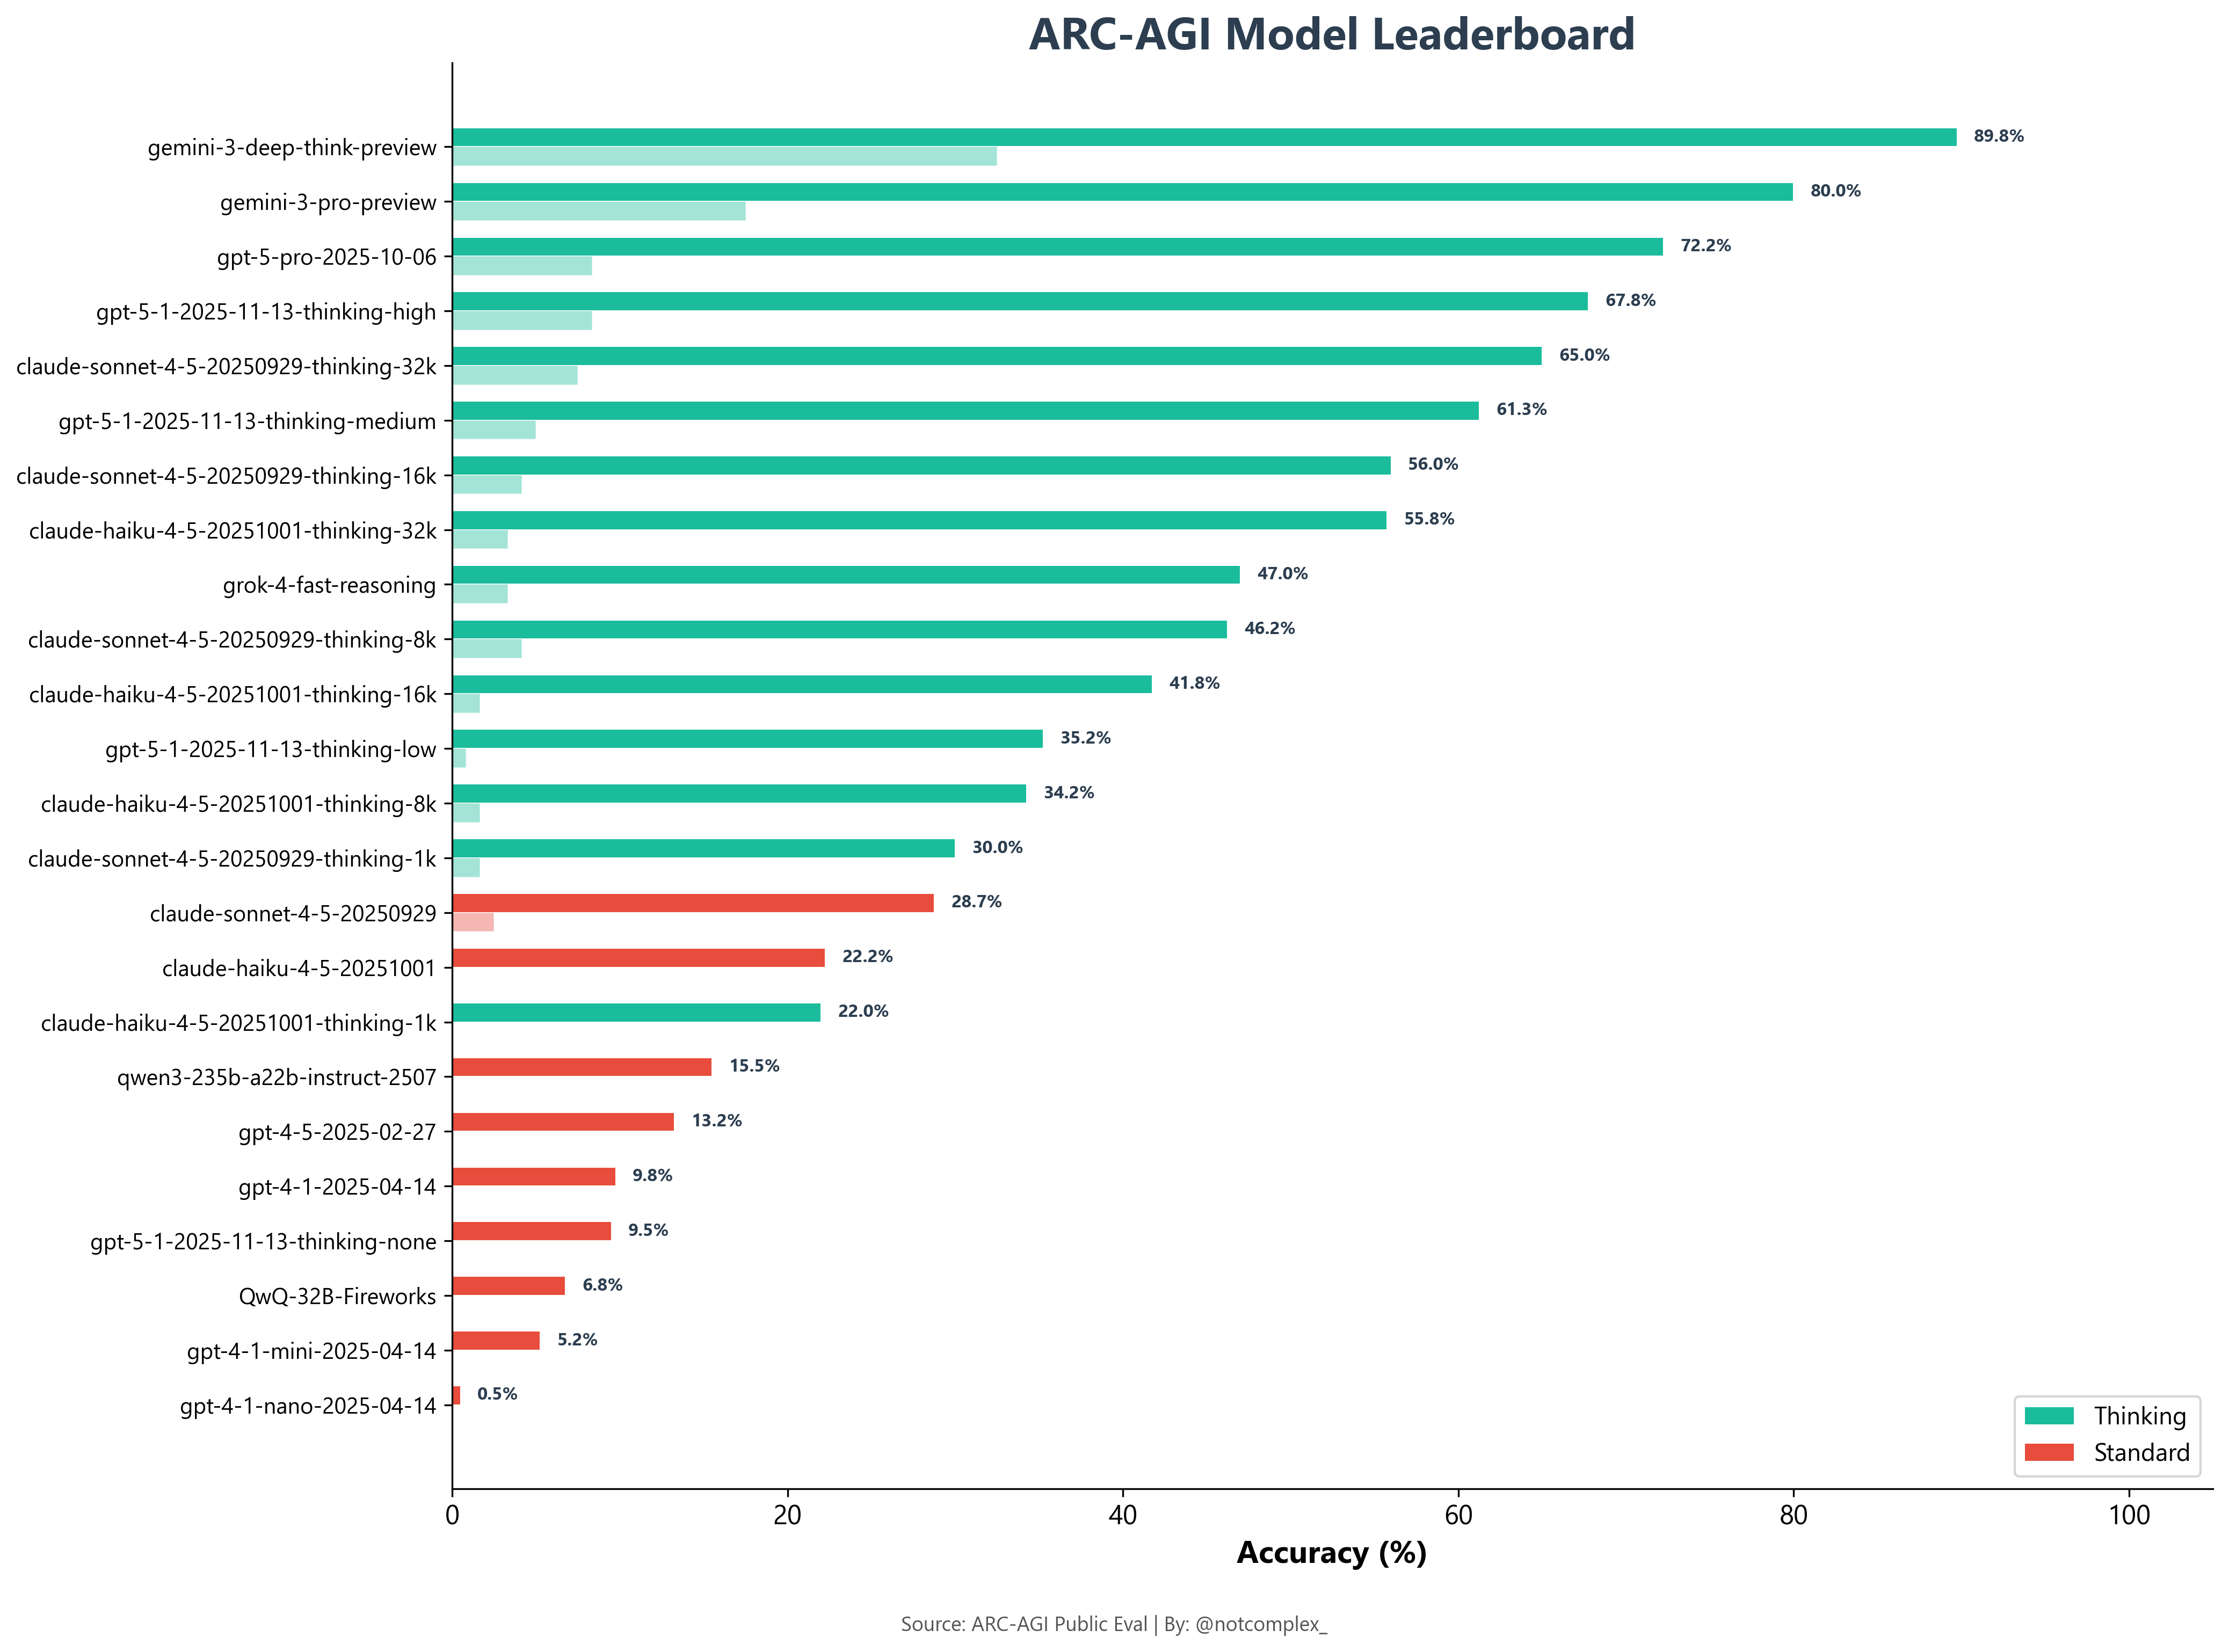
\includegraphics[width=\textwidth]{fig1_leaderboard.png}
    \caption{ARC-AGI leaderboard view from the LLM psychometric package. ARC-AGI-2 is not merely a small upward shift from ARC-AGI-1; it is dramatically harder even for the strongest models.}
\end{figure}

\begin{figure}[H]
    \centering
    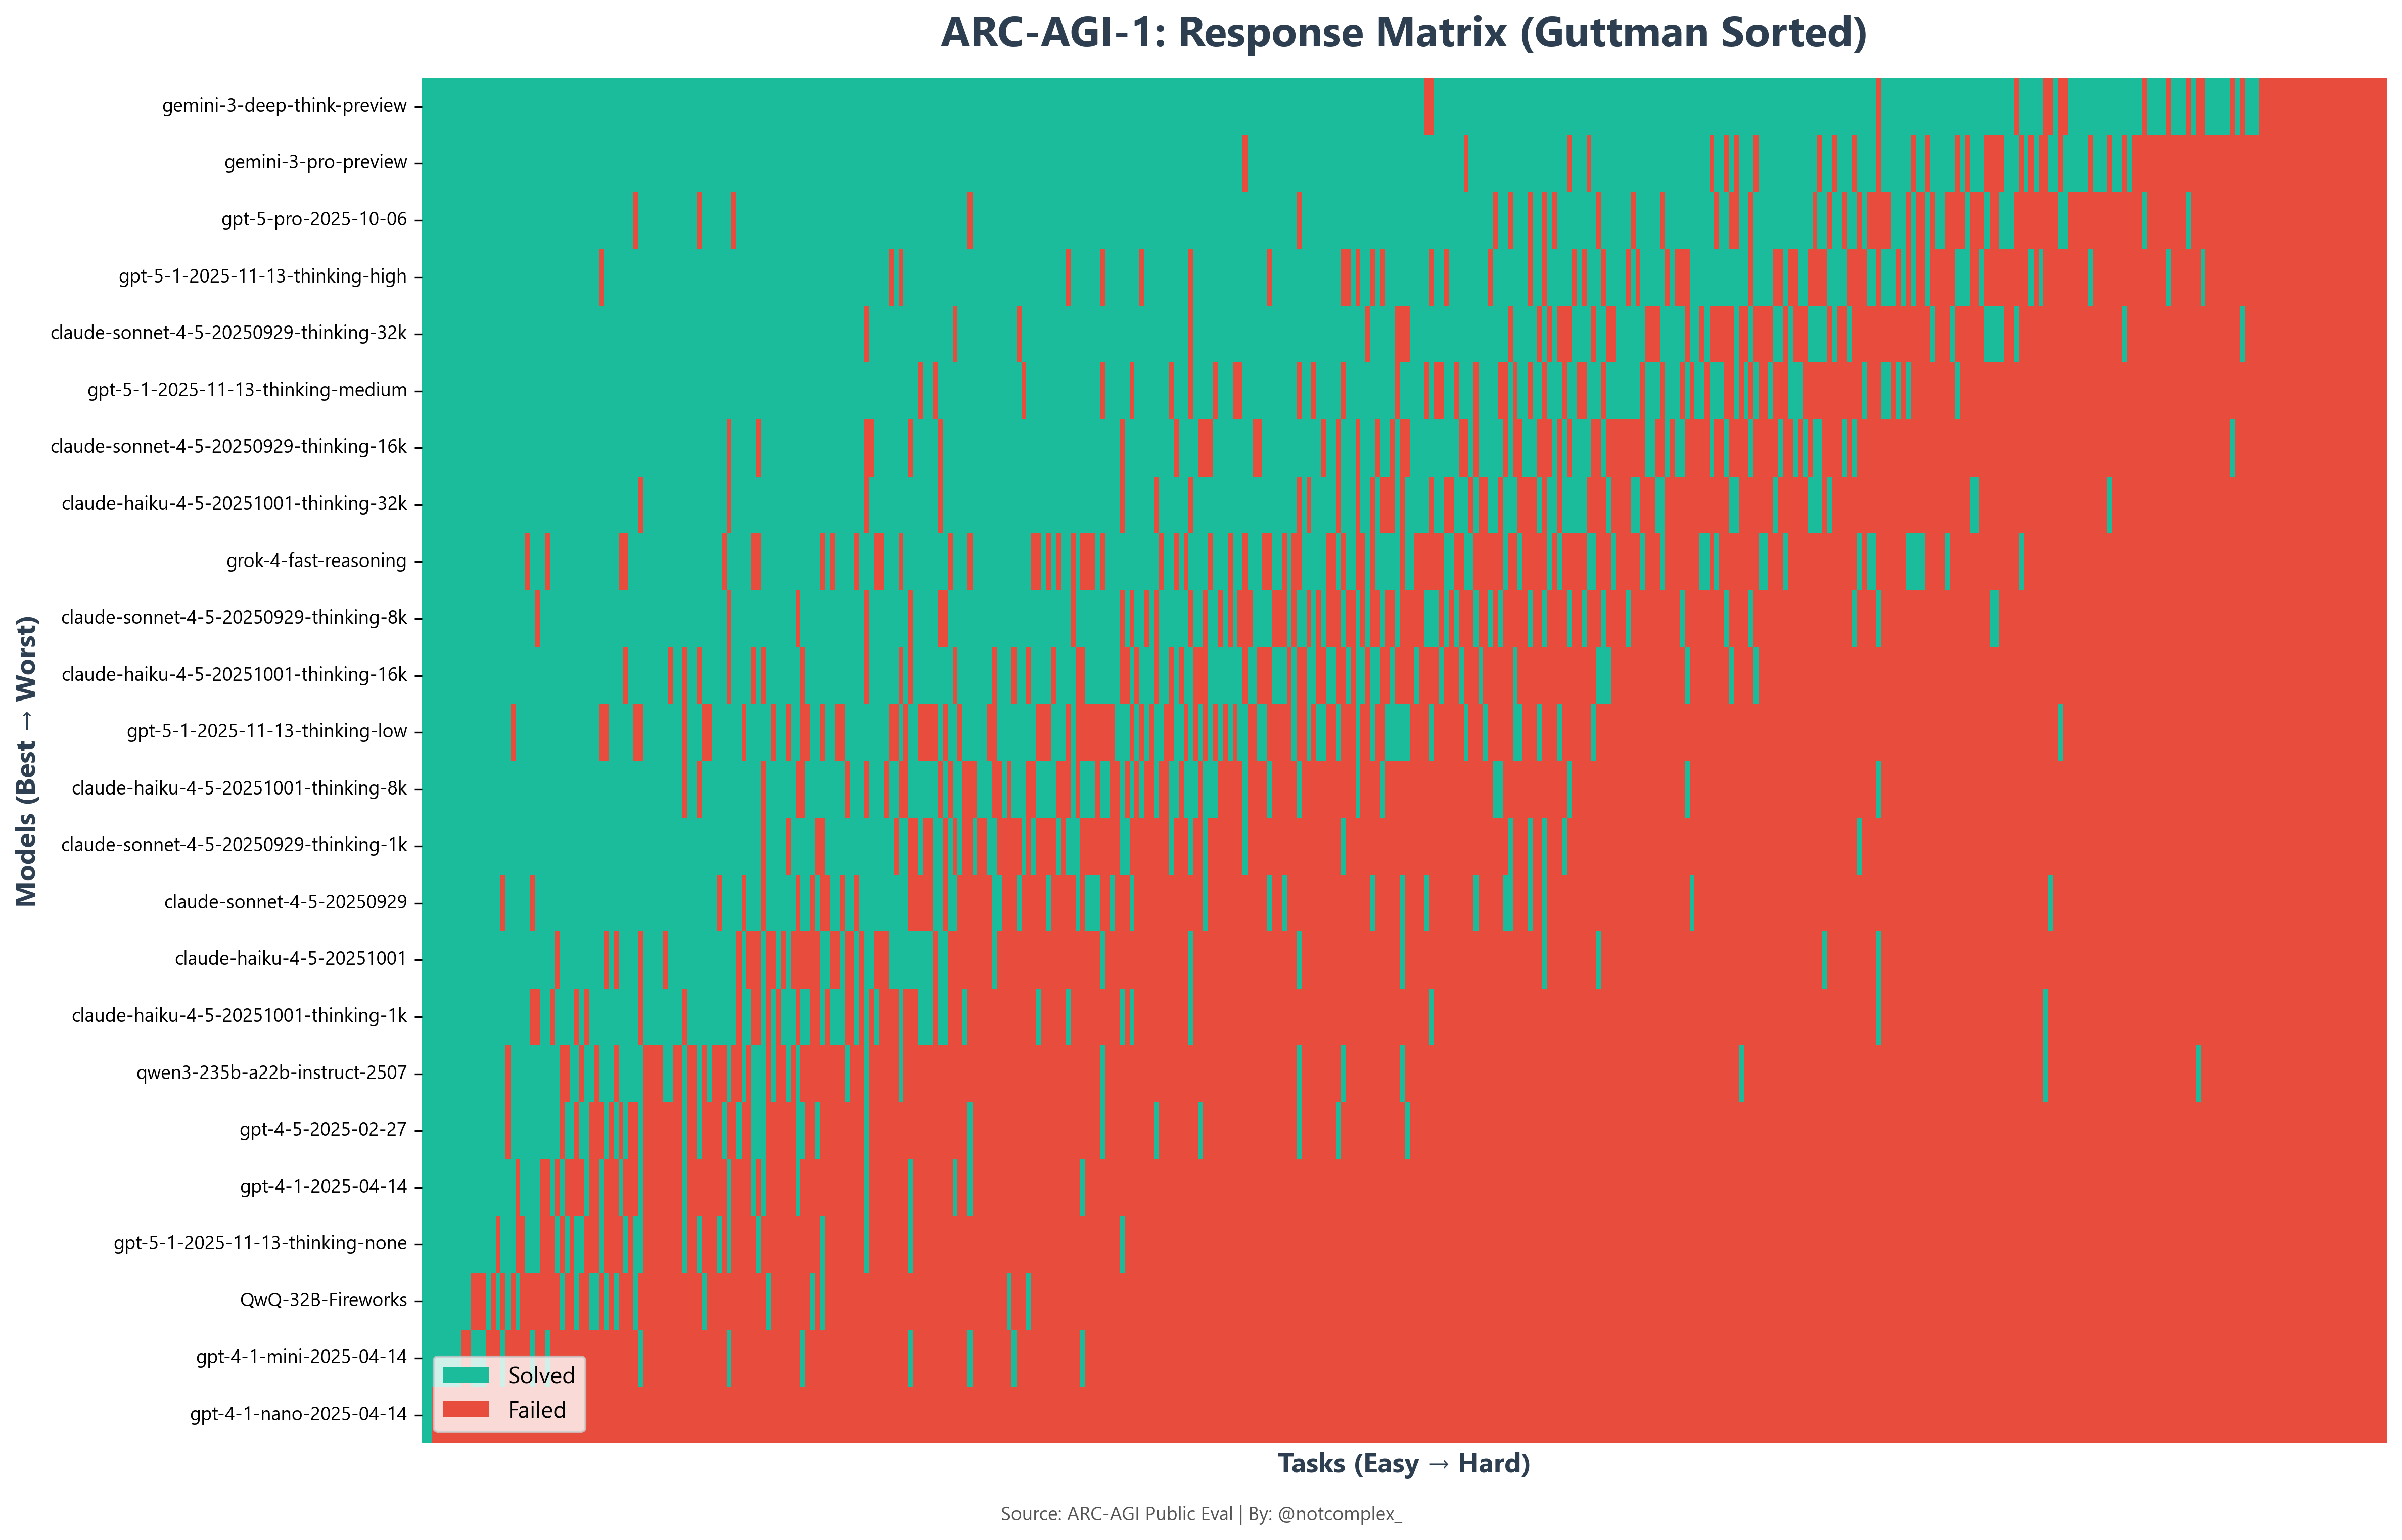
\includegraphics[width=\textwidth]{fig2_response_matrix_v1.png}
    \caption{ARC-AGI-1 response matrix sorted by model score and task pass rate. The staircase pattern is the visual signature of a cumulative difficulty structure rather than a patchwork of unrelated wins.}
\end{figure}

\begin{figure}[H]
    \centering
    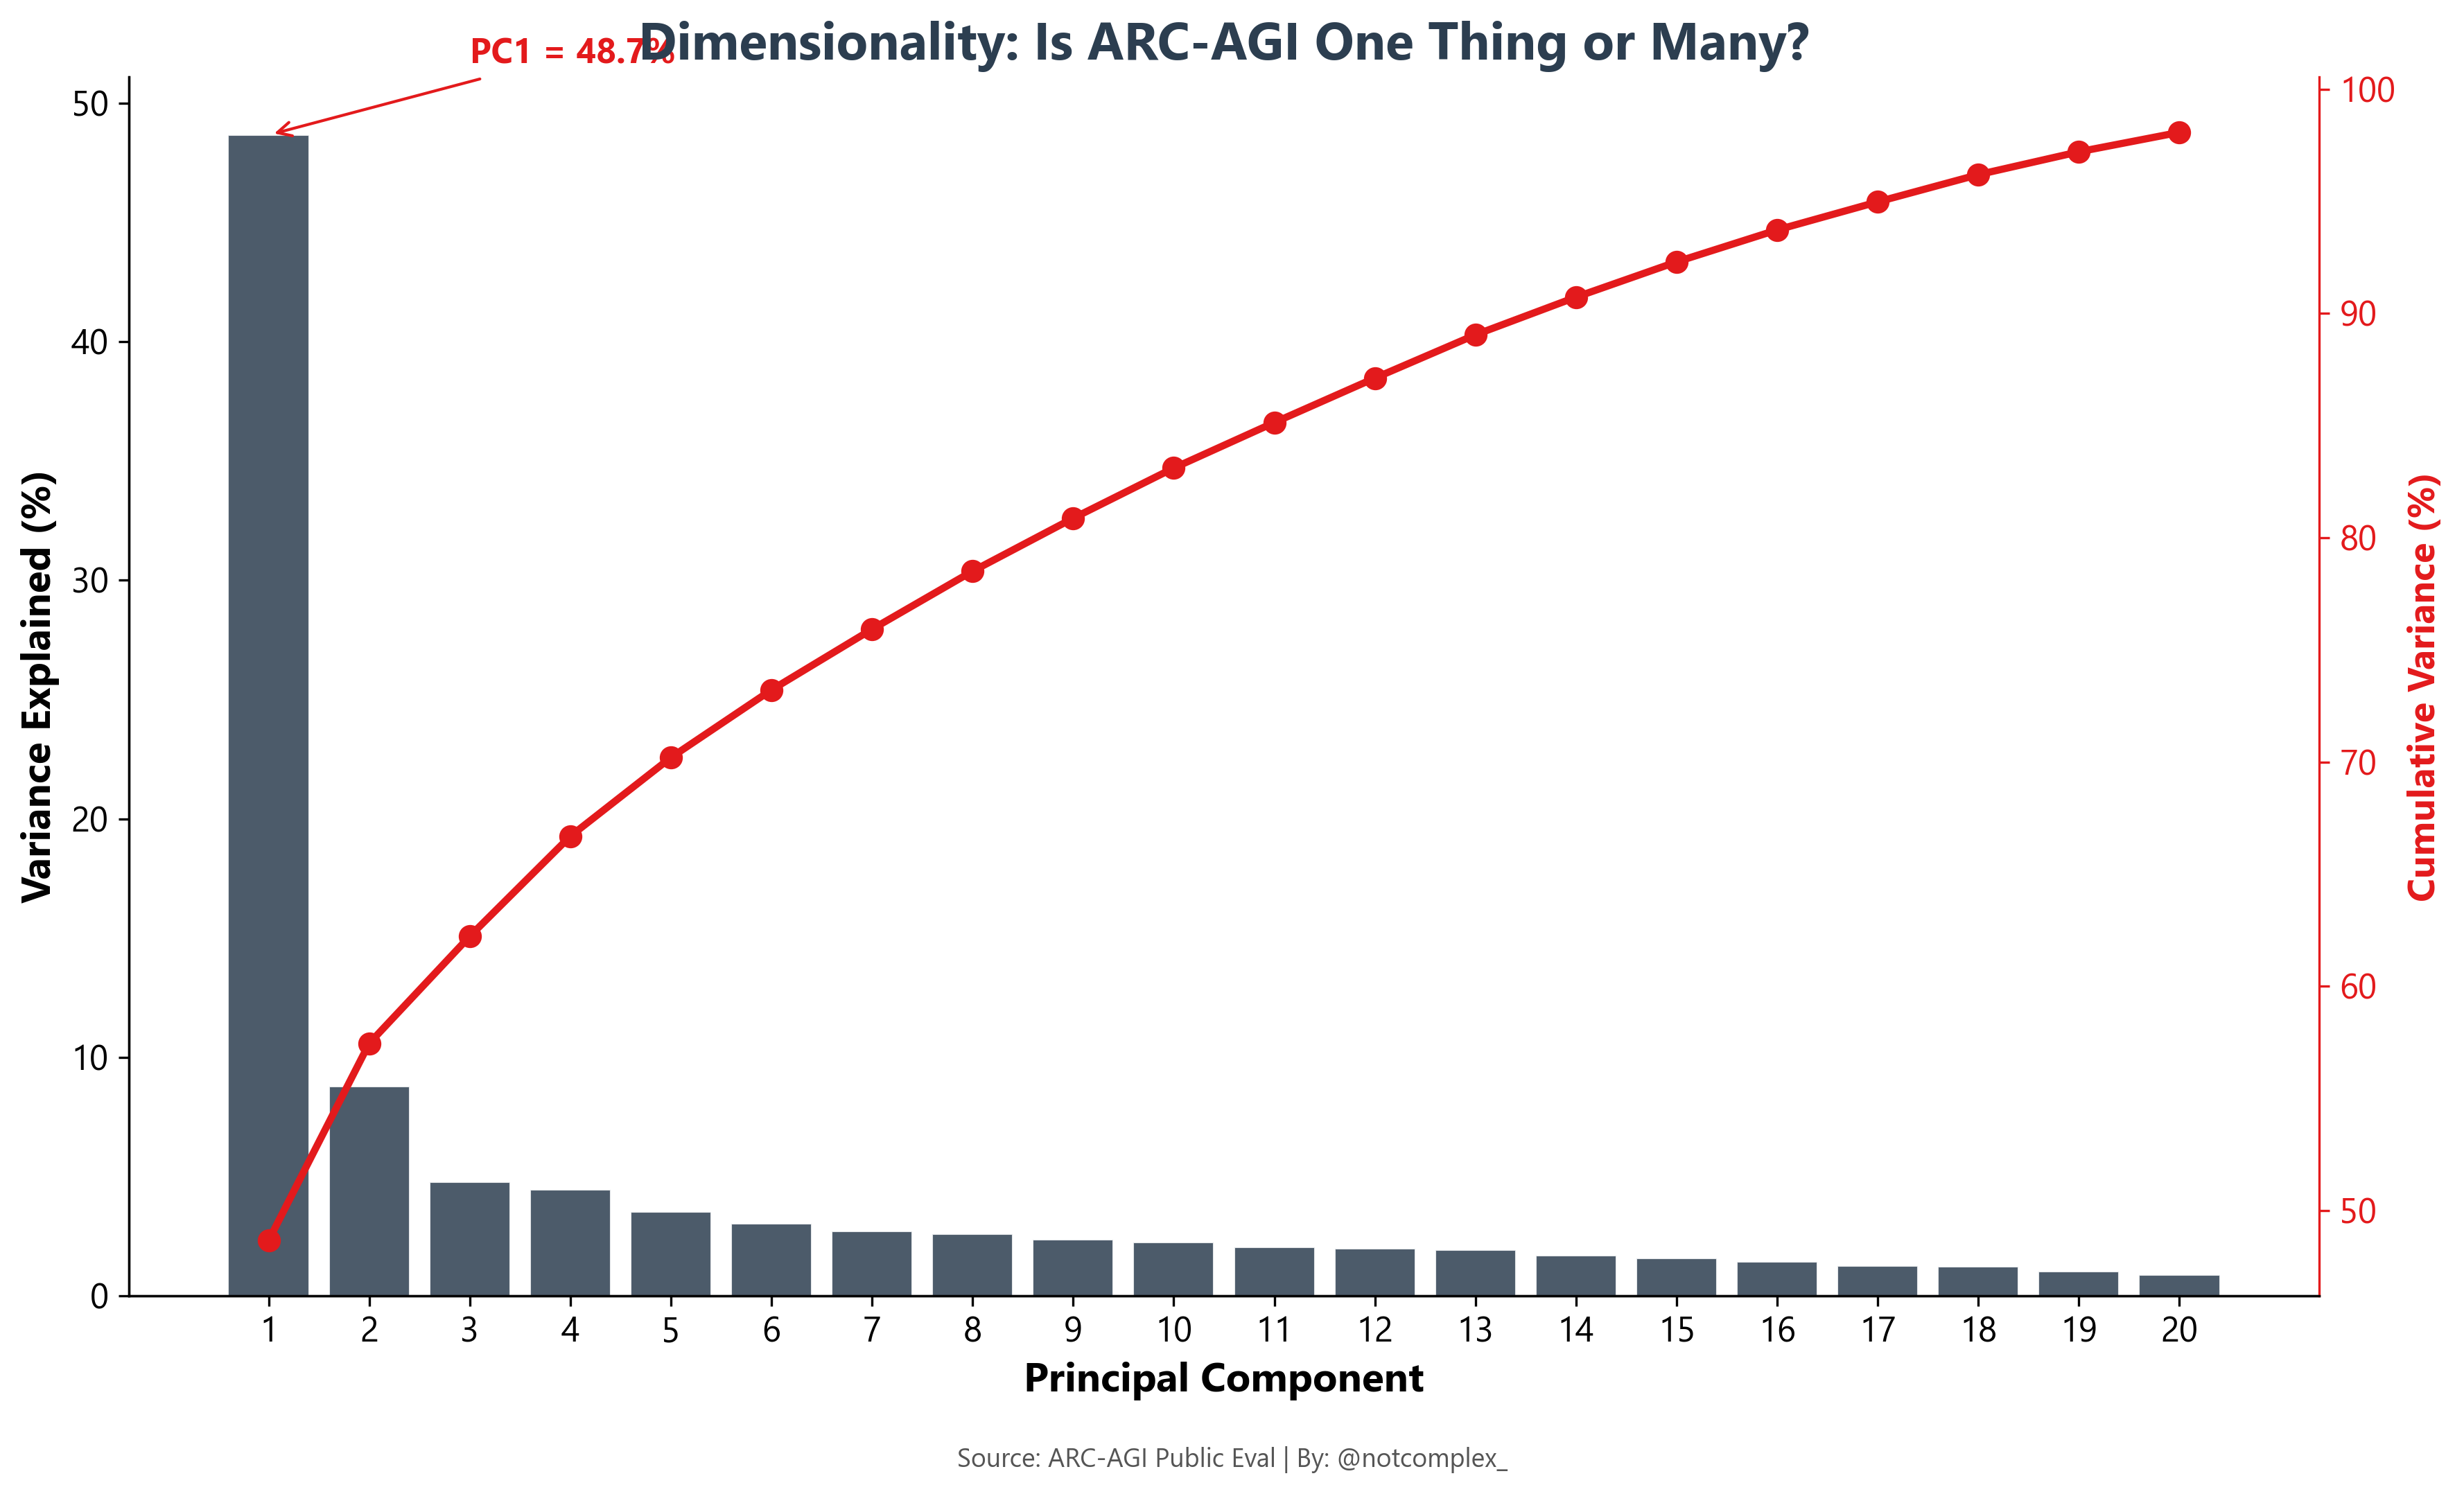
\includegraphics[width=0.9\textwidth]{fig3_scree_plot.png}
    \caption{Scree plot for the main ARC-AGI-1 model-by-task matrix. The large PC1-to-PC2 gap is the core reason the repository treats ARC as strongly one-factor dominated on the LLM side.}
\end{figure}

\begin{figure}[H]
    \centering
    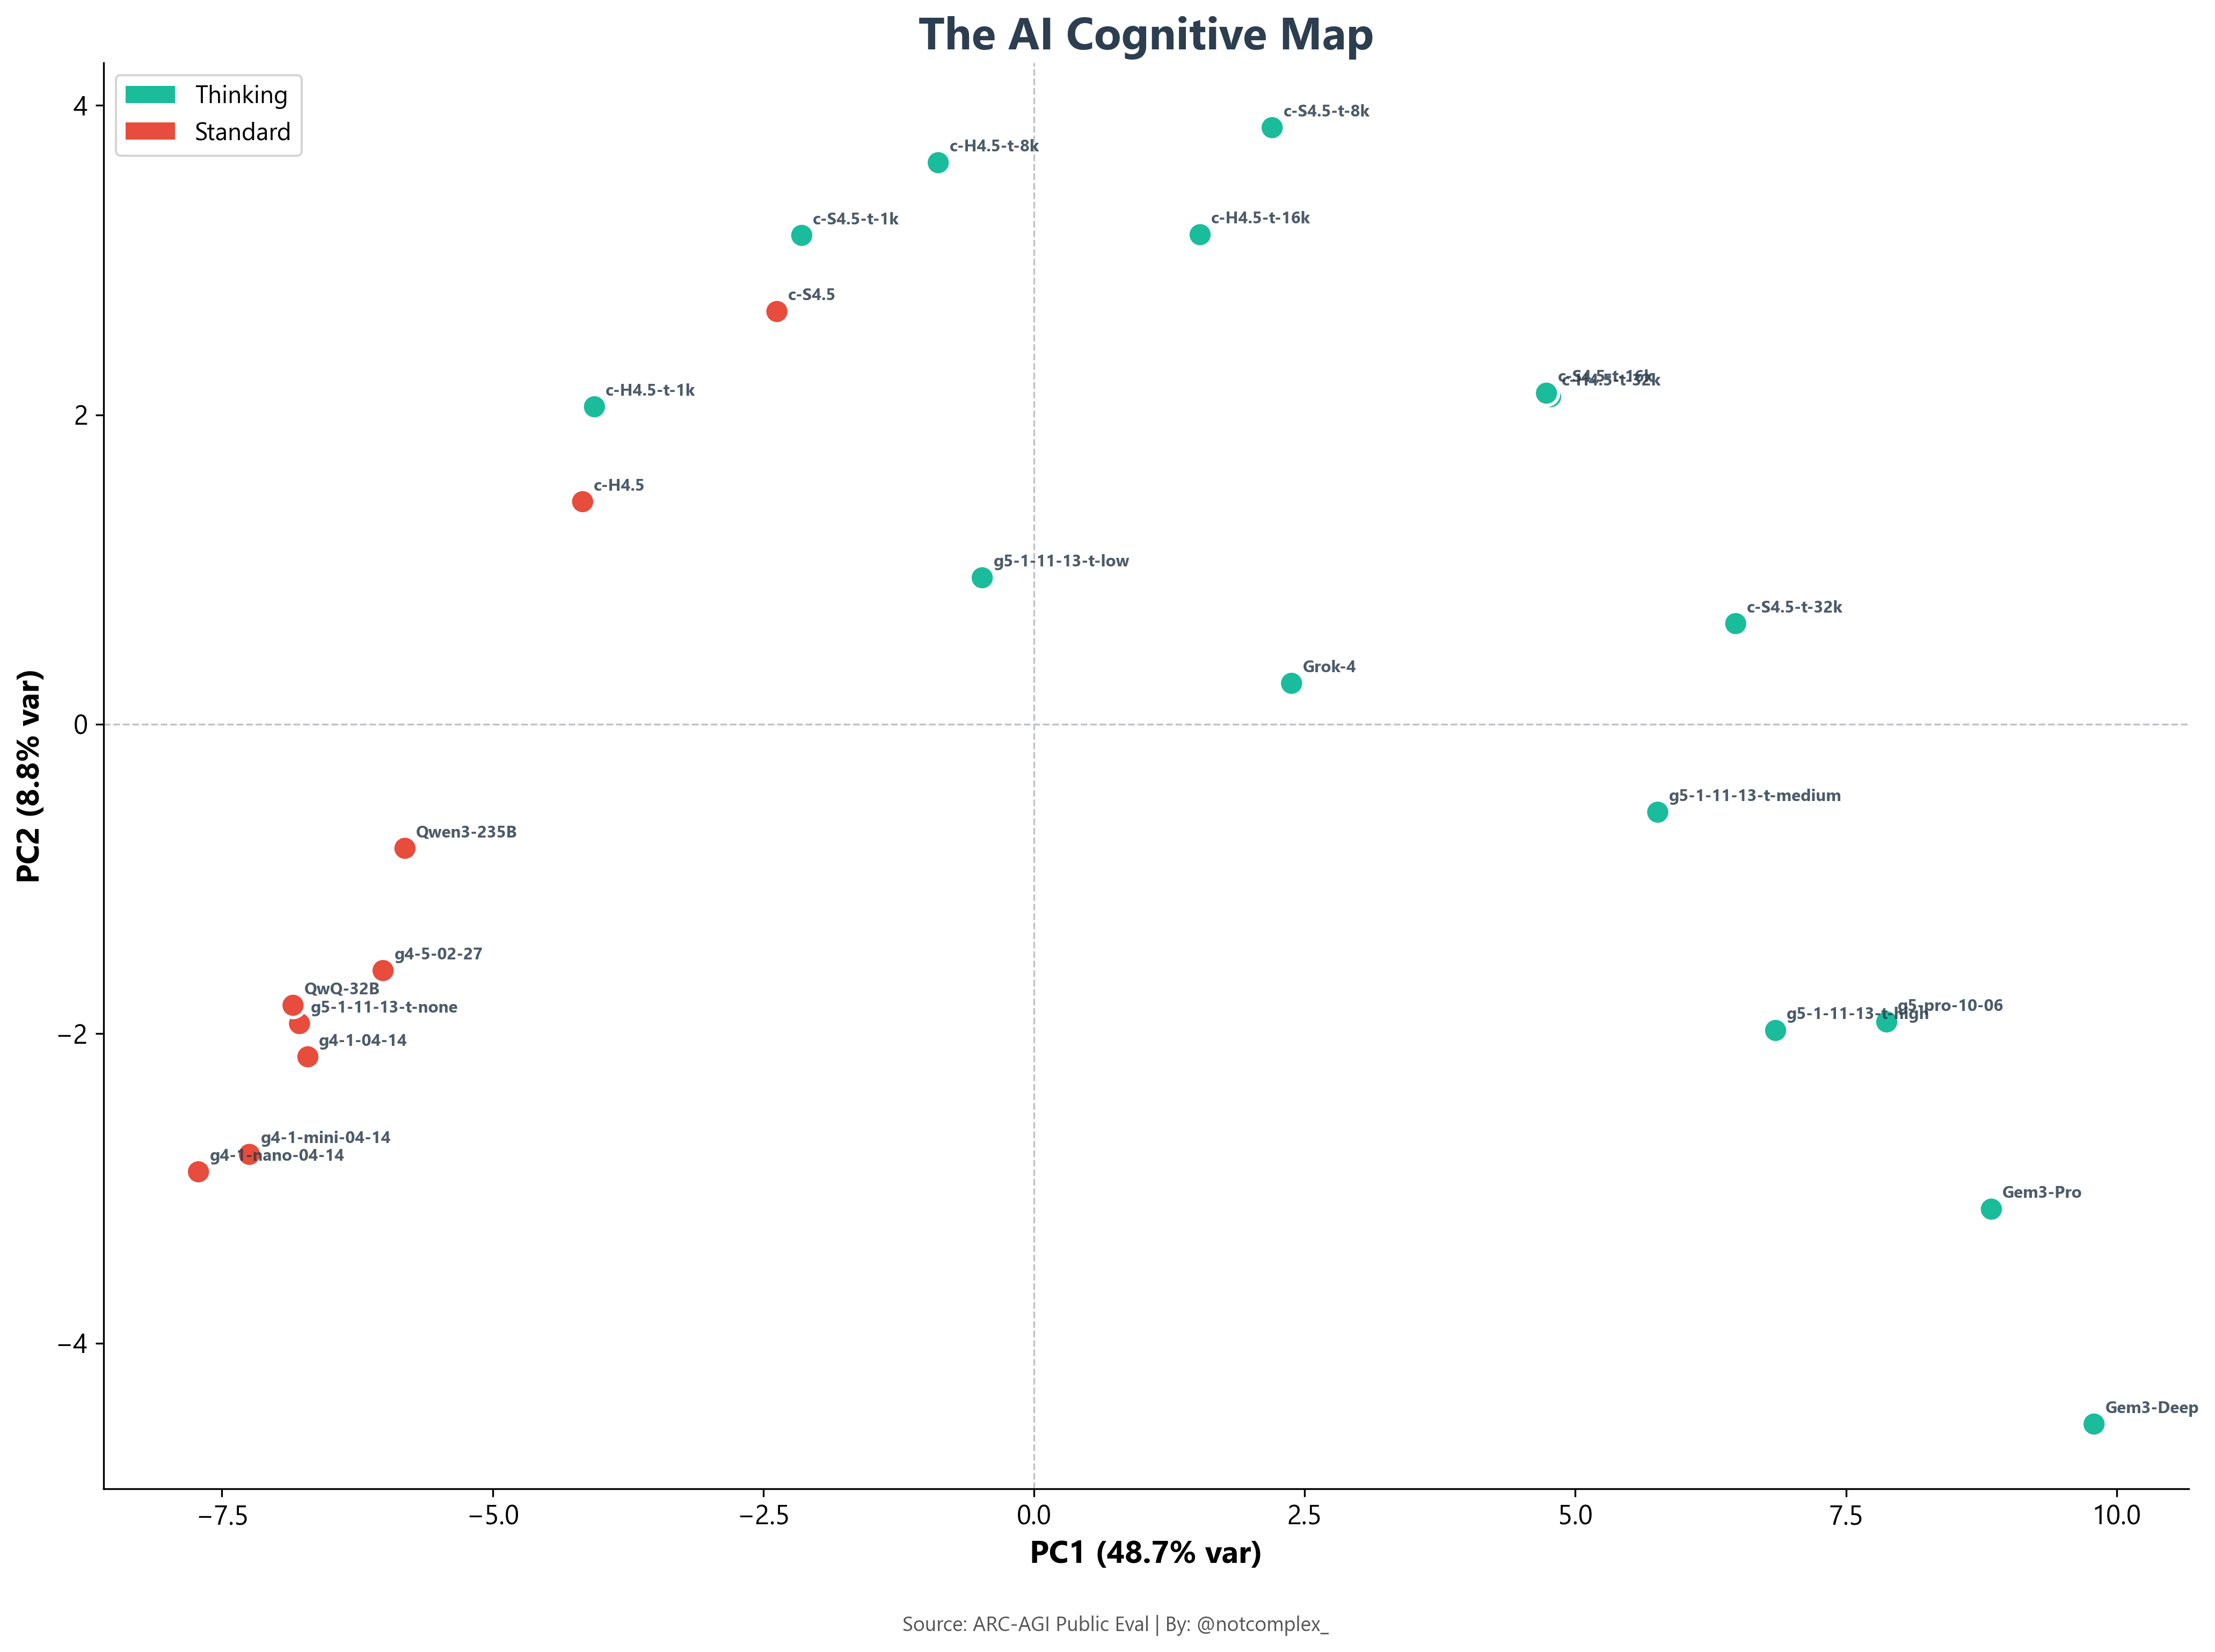
\includegraphics[width=0.92\textwidth]{fig4_cognitive_map.png}
    \caption{Low-dimensional cognitive map of the frontier model matrix. The key visual pattern is that stronger thinking variants extend the same main axis more than they open a qualitatively separate cluster.}
\end{figure}

\begin{figure}[H]
    \centering
    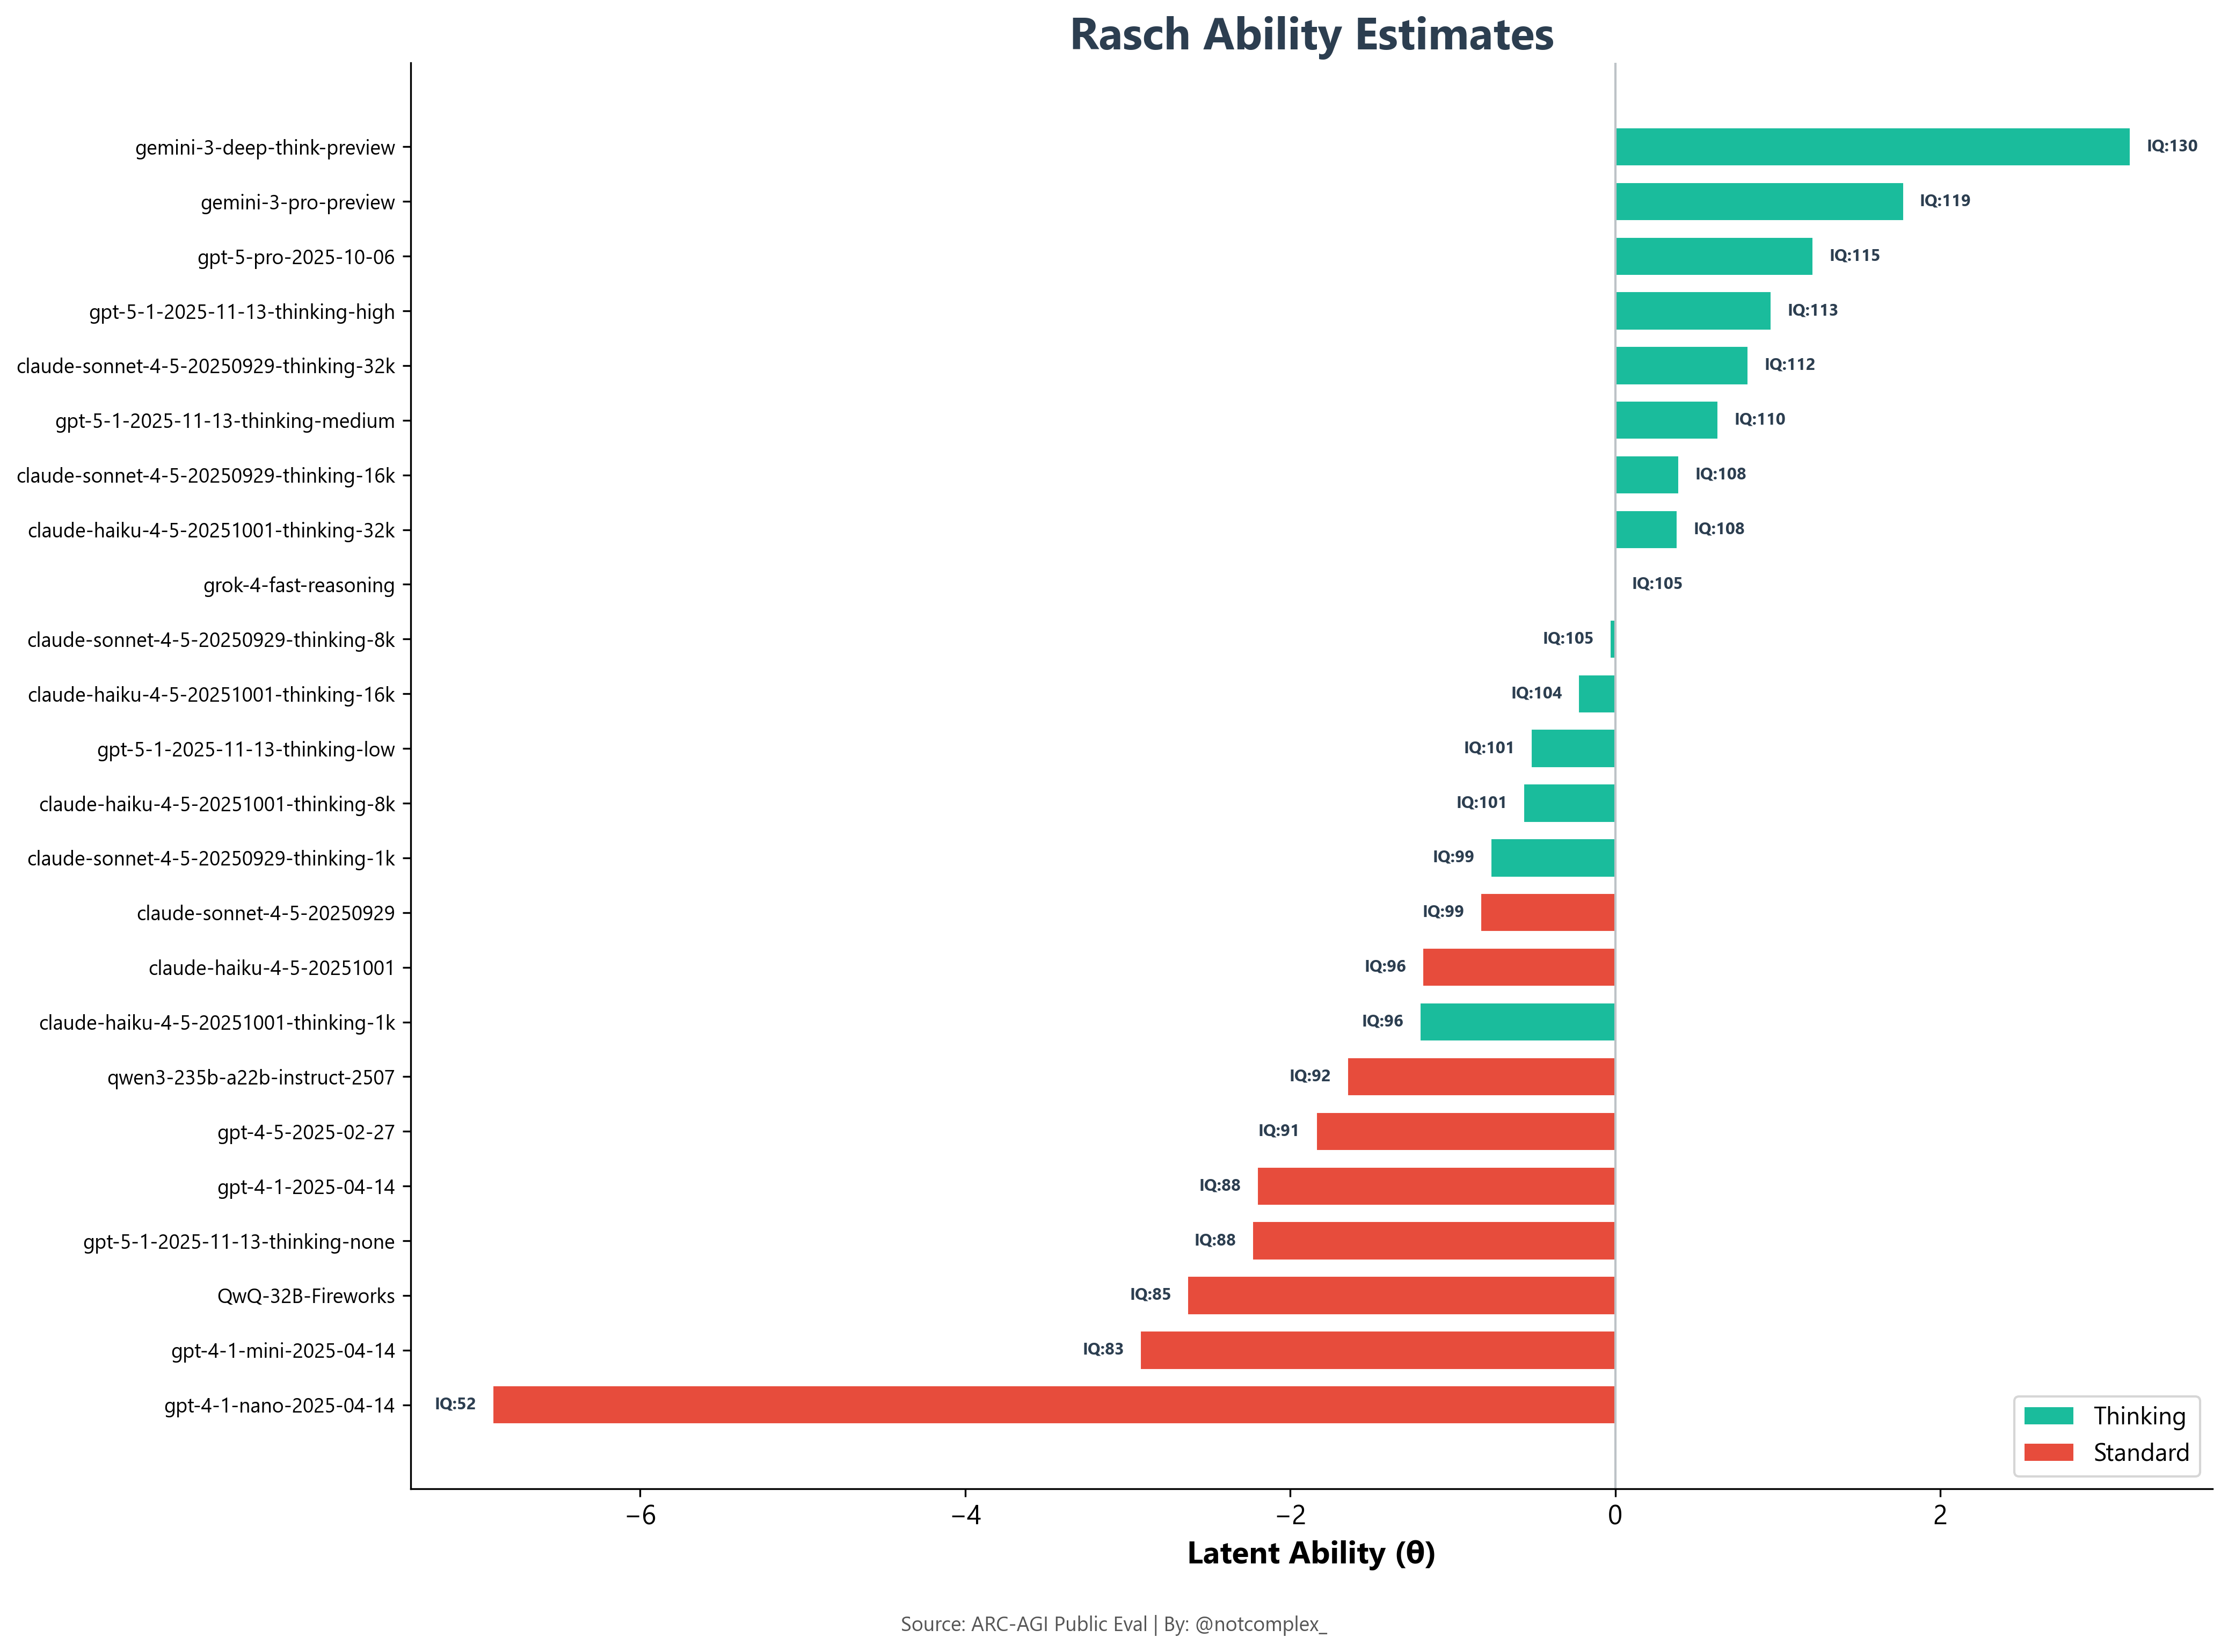
\includegraphics[width=0.88\textwidth]{fig5_ability.png}
    \caption{Estimated model ability under the main latent-difficulty fit. This is one of the views that makes the machine-side ARC scale usable for later comparison rather than just leaderboard reporting.}
\end{figure}

\subsection{Why this section matters for the rest of the paper}

The main contribution of the LLM psychometric line is not just that it supplies a leaderboard. It establishes the baseline against which the rest of the repository is interpreted. Human alignment matters because the model-side benchmark is not psychometrically chaotic. Solver-complexity correlations matter because LLM difficulty is stable across multiple difficulty constructions. Non-LLM comparisons matter because the benchmark already has a visible machine-side backbone, so failure to align with humans cannot be blamed on ARC itself being structureless.

% ===== Human Psychometrics =====
\section{Human Psychometrics}

\subsection{Goal}

The goal of the human workstream was to establish whether the sparse ARC human dataset is good enough to serve as a benchmark at all, and if so, what kind of benchmark it is. A second goal was to calibrate how much agreement we should expect between humans and models given the dataset's own internal noise.

\subsection{Data}

The human attempt log contains 4,681 attempts across 509 sessions, 442 observed task IDs, and 502 task-pair rows. Coverage is sparse and opportunistic rather than exam-like: only 40.4\% of ARC-AGI-2 public task pairs appear in the observed table, and the implied session-by-item matrix density is about 1.83\%. Public Train is easier than Public Eval, but Public Eval is the main overlap region for cross-system comparison.

\subsection{Methods}

The human pipeline combines descriptive solve-rate summaries with person-plus-item logistic modeling, split-half simulation, and later latent task estimation in the cross-ARC package. The key methodological move is to treat split-half human-versus-human correlations as the reference distribution for how large any human-versus-model correlation can realistically be on this sparse benchmark. This keeps later model comparisons from being judged against an unrealistic ceiling.

\subsection{Experiment}

The human line effectively ran three experiments. First, it tested whether the sparse human matrix still supports meaningful psychometric estimation. Second, it measured human split-half reproducibility on the public-eval overlap used for cross-system comparison. Third, it compared human item difficulty to several model-side profiles: the average model, the best single model, and a per-pair oracle profile.

\subsection{Results}

The basic result is that the human benchmark is noisy but usable. The held-in diagnostics for the person-plus-item model are strong enough to support latent estimation, and the cross-ARC package later shows that latent task scores are more stable than raw task means. The benchmark is sparse enough that the raw matrix itself matters: 4,681 attempts cover only 502 task-pair rows and about 40.4\% of public ARC-2 task pairs, so the paper cannot treat the human data like a complete exam matrix.

On the public-eval overlap, the human split-half median Pearson correlation is about 0.399. Human versus average-model correlation is about 0.402, which lands near the center of the human split-half distribution. Human versus best single model is lower, around 0.276, and human versus per-pair oracle sits in between, around 0.343. This leads to a balanced reading. The strongest version of ``models are random with respect to humans'' is not supported, because the average-model profile clearly aligns with human item difficulty. But the strongest version of ``leaderboard success means human-like ordering'' is also not supported, because even a strong single model does not line up with humans as well as one split-half of humans lines up with the other.

The data composition tables and figures also clarify what kind of benchmark this is. Attempted items are not representative: on Public Eval, attempted items average about 425 input cells versus about 269 for unattempted items. Human burden is also distinctive. Human difficulty is much more associated with duration than with raw board size, and within-task pair-level heterogeneity is substantial. These features become crucial later when the paper asks why solver complexity predicts LLM difficulty more strongly than human difficulty.

\begin{table}[H]
\centering
\small
\caption{Human benchmark snapshot from the unified attempt log. These values are the reason later sections lean on latent estimation and split-half benchmarking instead of treating raw human means as fully settled.}
\begin{tabular}{p{3.2in}p{1.5in}}
\toprule
\textbf{Quantity} & \textbf{Value} \\
\midrule
Attempts & 4,681 \\
Sessions & 509 \\
Observed task IDs & 442 \\
Observed task-pair rows & 502 \\
Task-pair coverage of all observed ARC pairs & 40.4\% \\
Implied session-by-item matrix density & 1.83\% \\
Overall solve rate & 75.3\% \\
Public Train solve rate & 80.4\% \\
Public Eval solve rate & 61.3\% \\
Median attempts per session & 8 \\
Median attempts per item & 9 \\
\bottomrule
\end{tabular}
\end{table}

\begin{table}[H]
\centering
\scriptsize
\caption{Sampling-bias summary from the human-testing package. Attempted items are consistently larger than unattempted items, especially on Public Eval.}
\begin{tabular}{p{1.0in}p{0.9in}p{0.55in}p{0.8in}p{0.8in}p{0.8in}}
\toprule
\textbf{Task set} & \textbf{Status} & \textbf{$n$} & \textbf{Mean input cells} & \textbf{Mean colors} & \textbf{Mean train pairs} \\
\midrule
Public Eval & Unattempted & 5 & 269.2 & 6.30 & 3.60 \\
Public Eval & Attempted & 115 & 424.8 & 5.45 & 2.97 \\
Public Train & Unattempted & 674 & 145.9 & 3.75 & 3.23 \\
Public Train & Attempted & 326 & 293.1 & 4.36 & 3.24 \\
\bottomrule
\end{tabular}
\end{table}

\begin{table}[H]
\centering
\scriptsize
\caption{Human-versus-model alignment in the public-eval overlap, benchmarked against human split-half reliability. Including the overlap-set Jaccard terms makes it clear that Pearson alone is not the only sense in which the average-model profile behaves human-like.}
\begin{tabular}{p{1.95in}p{0.7in}p{0.7in}p{0.7in}p{0.7in}p{0.9in}}
\toprule
\textbf{Series} & \textbf{Pearson $r$} & \textbf{Spearman $\rho$} & \textbf{Hard Jacc.} & \textbf{Easy Jacc.} & \textbf{Percentile vs split-half} \\
\midrule
Human split-half median & 0.399 & 0.427 & 0.135 & 0.235 & 0.500 \\
Human vs average model & 0.402 & 0.454 & 0.100 & 0.419 & 0.523 \\
Human vs best single model & 0.276 & 0.276 & 0.000 & 0.257 & 0.023 \\
Human vs per-pair oracle & 0.343 & 0.346 & 0.100 & 0.375 & 0.179 \\
\bottomrule
\end{tabular}
\end{table}

\begin{figure}[H]
    \centering
    \includegraphics[width=\textwidth]{fig01_human_response_matrix.png}
    \caption{Observed human response matrix from the human-testing package. The missingness pattern is part of the result: this is a sparse, opportunistic human benchmark rather than a cleanly administered test.}
\end{figure}

\begin{figure}[H]
    \centering
    \includegraphics[width=0.92\textwidth]{fig05_sampling_bias.png}
    \caption{Sampling-bias visualization from the human package. The paper needs this view because later cross-system claims are otherwise easy to over-read as if humans saw a representative subset.}
\end{figure}

\begin{figure}[H]
    \centering
    \includegraphics[width=0.92\textwidth]{fig01_split_half_vs_models.png}
    \caption{Split-half context against human-versus-model correlations. This is the most direct visual reason the paper treats the average-model alignment result as real but incomplete.}
\end{figure}

\begin{figure}[H]
    \centering
    \includegraphics[width=0.92\textwidth]{human_split_half_stability.png}
    \caption{Raw solve rates versus latent task estimates under split-half resampling in the cross-ARC package. The main point is that latent task estimates are more stable than naive raw means in every benchmark slice.}
\end{figure}

\begin{figure}[H]
    \centering
    \includegraphics[width=0.92\textwidth]{fig07_human_vs_lm_public_eval.png}
    \caption{Public-eval human-versus-model comparison view from the human-testing package. The figure complements the table by showing where the average-model profile does and does not overlap the human ordering.}
\end{figure}

\subsection{Why this section matters for the rest of the paper}

The human workstream is what forces the paper to distinguish shared difficulty from shared burden. Without it, ARC could be narrated as a clean machine psychometric instrument. With it, the paper has to deal with sparse exposure, moderate reliability, duration, and pair-level heterogeneity. Those are not side issues; they are the empirical reasons the full manuscript ends up arguing that humans and models overlap on one difficulty axis while diverging on what makes a task burdensome.

% ===== Non-LLM Psychometrics =====
\section{Non-LLM Psychometrics}

\subsection{Goal}

The goal of the non-LLM workstream was not just to collect alternative ARC scores. It was to ask a sharper question: once we add bona fide non-LLM systems to the repo, do they look more human-like than the LLM aggregate, less human-like, or simply different in a complementary way?

\subsection{Data}

The main comparison space is ARC-AGI-2 Public Eval because that is where the human attempt data and stored prediction corpora overlap cleanly. The primary subset contains 110 public-eval test pairs with at least 8 human attempts each. The main non-LLM sources are TRM ARC-AGI-II evaluator submissions and VARC ARC-2 prediction dumps. CompressARC contributes an ARC-1 sidecar rather than a direct ARC-2 comparison.

\subsection{Methods}

The non-LLM section uses more than one null because low-score binary systems are easy to misread. It benchmarks systems against the human split-half distribution, reruns the analysis at several human-attempt thresholds, tests fixed-accuracy random-placement nulls, controls for simple task features, compares against accuracy-matched weak LLMs, and checks for residual signal after controlling the LLM average. It also looks for complementarity by asking whether non-LLM systems rescue human-easy and LLM-hard items above chance.

\subsection{Experiment}

The core experiment compares several selected profiles on the same ARC-2 human-overlap subset: the LLM average, the best-aligned single LLM, the best-score single LLM, a mid-training TRM checkpoint, a later higher-score TRM checkpoint, and the strongest stored VARC ARC-2 profile. The follow-up experiments then ask whether low raw correlations are better than score-matched random placement, whether any residual human-like structure survives simple controls, and whether TRM training improves human-likeness or only score.

\subsection{Results}

The top line is disappointing but clear. The LLM average reaches a human-correlation value around 0.402 on the primary 110-pair subset, while the best-aligned single LLM reaches about 0.439. The most human-aligned TRM checkpoint reaches only about 0.214, and the best VARC profile about 0.158. Human-equivalence is not rejected for the LLM average or the best-aligned LLM, but it is rejected for the leading non-LLM profiles.

At the same time, raw correlation is not the whole story. The threshold-sensitivity table shows that the ordering is stable as the human-attempt filter tightens: the LLM aggregate and the best-aligned single LLM improve steadily, while TRM and VARC remain well below them. The mid-training TRM checkpoint exceeds the same-accuracy random-placement null, whereas the later best-score TRM checkpoint does not. TRM and VARC also rescue a handful of human-easy and LLM-hard items, and the TRM plus VARC union rescues 6 such items above chance. So the non-LLM systems are not useless or redundant; they are simply weaker than hoped as broad human-profile matches.

\begin{table}[H]
\centering
\small
\caption{Headline ARC-2 results for selected LLM and non-LLM profiles on the 110-pair primary subset.}
\begin{tabular}{p{2.45in}p{0.8in}p{0.9in}p{0.8in}}
\toprule
\textbf{Profile} & \textbf{Pair Acc.} & \textbf{Human $r$} & \textbf{H1 $p$} \\
\midrule
LLM average & 0.108 & 0.402 & 0.950 \\
Best-aligned LLM (Claude Opus 16k) & 0.164 & 0.439 & 0.506 \\
Best-score LLM (GPT-5-2 xhigh) & 0.491 & 0.276 & 0.052 \\
TRM 361957 pass@2 & 0.045 & 0.214 & 0.004 \\
TRM 651522 pass@2 & 0.109 & 0.113 & 0.0004 \\
VARC ARC-2 ViT pass@2 & 0.036 & 0.158 & 0.0004 \\
\bottomrule
\end{tabular}
\end{table}

\begin{table}[H]
\centering
\scriptsize
\caption{Threshold sensitivity on the ARC-2 public-eval overlap. Tightening the human-attempt filter changes the absolute values but not the broad ordering.}
\begin{tabular}{p{0.55in}p{0.55in}p{0.62in}p{0.62in}p{0.62in}p{0.62in}p{0.62in}p{0.62in}}
\toprule
\textbf{Min attempts} & \textbf{$n$ pairs} & \textbf{LLM avg} & \textbf{Opus 16k} & \textbf{GPT-5.2 xh} & \textbf{TRM 361957} & \textbf{TRM 651522} & \textbf{VARC ViT} \\
\midrule
2 & 161 & 0.345 & 0.348 & 0.256 & 0.164 & 0.090 & 0.091 \\
3 & 159 & 0.351 & 0.362 & 0.242 & 0.171 & 0.098 & 0.096 \\
5 & 129 & 0.367 & 0.403 & 0.231 & 0.199 & 0.095 & 0.142 \\
8 & 110 & 0.402 & 0.439 & 0.276 & 0.214 & 0.113 & 0.158 \\
\bottomrule
\end{tabular}
\end{table}

\begin{table}[H]
\centering
\small
\caption{Complementary rescue of human-easy and LLM-hard pairs. This is the compact reason the paper keeps a non-redundancy claim even while rejecting strong human-equivalence claims.}
\begin{tabular}{p{2.2in}p{0.8in}p{0.8in}p{0.9in}p{0.8in}}
\toprule
\textbf{System} & \textbf{Solved items} & \textbf{Rescued pairs} & \textbf{Random expectation} & \textbf{$p$} \\
\midrule
TRM 651522 pass@2 & 12 & 5 & 2.4 & 0.061 \\
VARC ARC-2 ViT pass@2 & 4 & 3 & 0.8 & 0.025 \\
TRM + VARC union & 13 & 6 & 2.6 & 0.022 \\
\bottomrule
\end{tabular}
\end{table}

\begin{figure}[H]
    \centering
    \includegraphics[width=0.92\textwidth]{fig02_threshold_sensitivity.png}
    \caption{Threshold-sensitivity figure from the non-LLM package. The ranking is stable enough that the paper can treat the disappointing non-LLM result as robust rather than a threshold artifact.}
\end{figure}

\begin{figure}[H]
    \centering
    \includegraphics[width=0.92\textwidth]{fig09_alignment_band.png}
    \caption{Selected ARC-2 system profiles against the human split-half benchmark. The visual point is simple: the LLM aggregate sits inside the human split-half band, while the current non-LLM systems do not.}
\end{figure}

\begin{figure}[H]
    \centering
    \includegraphics[width=0.92\textwidth]{fig10_fixed_accuracy_null.png}
    \caption{Observed human-alignment against the fixed-accuracy random-placement null. This is the key correction for score sparsity: low raw correlation can still be meaningful if it beats what random placement at the same number of wins would produce.}
\end{figure}

\begin{figure}[H]
    \centering
    \includegraphics[width=0.96\textwidth]{fig07_trm_trajectory.png}
    \caption{TRM training dynamics on the human-overlap subset. Score rises over training, but human-alignment peaks earlier and does not improve in lockstep.}
\end{figure}

\begin{figure}[H]
    \centering
    \includegraphics[width=0.92\textwidth]{fig11_residual_signal.png}
    \caption{Residual-signal view from the non-LLM package. The point is not that non-LLM systems broadly match humans, but that they retain some structure that is not exhausted by the LLM average.}
\end{figure}

\subsection{Why this section matters for the rest of the paper}

This section is where the repository's most disappointing result lives, and it is important precisely because the rest of the paper depends on not hiding it. Current non-LLM systems are not the clean human-like alternative to the LLM consensus on the available psychometric evidence. But they are also not vacuous. They contribute complementary successes, they separate benchmark score from human-like item placement, and they set up the architectural question explored later in the paper: why do these systems seem mechanistically promising even while their current human-alignment numbers remain modest?

% ===== Solver Complexity =====
\section{Solver Complexity}

\subsection{Goal}

The goal of the solver-complexity line was to test the strongest integrative hypothesis in the repo: when ARC tasks require more structurally complex successful solvers, does that burden show up equally for humans, LLMs, and non-LLM systems, or does it load differently across source families?

\subsection{Data}

The starting point is a validated corpus of Python ARC solvers. A total of 511 \texttt{solution.py} files were fetched from \texttt{arc.huikang.dev}, but only 127 passed validation against the official ARC task files. The decisive filter turned out to be the site's approved label: 120 of 120 approved solvers passed. The main analysis therefore uses the 120-task approved-only package and joins it to human difficulty summaries, LLM difficulty summaries, and smaller non-LLM overlap slices.

\subsection{Methods}

The complexity panel includes static structural metrics such as token count, AST node count, branching, cyclomatic complexity, nesting depth, gzip bytes, and Halstead measures, plus dynamic runtime-style metrics such as opcode counts, Python call counts, elapsed time, and peak memory. The workstream uses PCA to summarize the panel, single-metric and composite correlations against difficulty summaries, paired difference-of-correlation tests, residualization to separate shared from source-specific burden, and later pooled benchmark-standardized extensions in the cross-ARC package.

\subsection{Experiment}

The main experiment ran in three layers. First, it asked whether the complexity panel is dominated by one structural axis or many unrelated ones. Second, it tested which complexity measures best predict LLM difficulty. Third, it asked whether the same measures predict human difficulty equally well on the matched overlap. Later addenda then stress-tested the result with residual analyses, softer output-closeness metrics, thinking-model audits, and pooled cross-ARC extensions.

\subsection{Results}

The first result is that the complexity panel is structured rather than arbitrary. PC1 explains 57.4\% of variance and behaves like overall solver size and structural density, while later components track runtime or footprint more weakly. The second result is that validated solver structure predicts LLM difficulty strongly. Earlier latent analyses found AST node count around $r = 0.666$ against latent difficulty, and the approved-only analysis found log-transformed cyclomatic complexity around $r = 0.707$ against simple LLM logit difficulty.

The third result is the most important in the whole repository. Humans and LLMs do share a real common difficulty axis on the approved overlap, with human difficulty versus LLM difficulty around $r = 0.531$ and human solve rate versus average-model pass rate around $r = 0.541$. But solver structure does not load equally on the two sides. Cyclomatic complexity correlates only weakly with human difficulty, about $r = 0.150$, while correlating much more strongly with LLM difficulty, about $r = 0.591$. The paired difference survives correction at about $\Delta r = 0.441$, with $p = 0.0378$ and $q = 0.0472$.

Residual analyses sharpen the same point. After removing shared human difficulty, residual LLM difficulty still tracks cyclomatic complexity at about $r = 0.603$. On the human side, the distinctive burden looks more duration- and search-like than structure-like. The human addenda reinforce that reading by showing that pair-level human difficulty tracks human duration much more strongly than raw board size and that within-task human heterogeneity is substantial. The audit table below is useful because it shows that the whole line is not hanging on one cherry-picked coefficient: the shared-alignment, difference, residual, and pair-level burden claims all survive as a coherent pattern.

\begin{table}[H]
\centering
\small
\caption{Key solver-complexity results carried into the master paper.}
\begin{tabular}{p{3.25in}p{1.6in}}
\toprule
\textbf{Quantity} & \textbf{Value} \\
\midrule
Fetched solver files & 511 \\
Validated solver files & 127 \\
Approved and validated solvers & 120 / 120 \\
Best single-metric LLM predictor (earlier latent line) & AST nodes, $r = 0.666$ \\
Best approved-only LLM predictor & $\log(1 + \mathrm{cyclomatic})$, $r = 0.707$ \\
Human difficulty vs LLM difficulty & $r = 0.531$ \\
Human solve rate vs LLM pass rate & $r = 0.541$ \\
Cyclomatic vs human difficulty & $r = 0.150$ \\
Cyclomatic vs LLM difficulty & $r = 0.591$ \\
Human-vs-LLM delta for cyclomatic & $\Delta r = 0.441$, $q = 0.0472$ \\
Residual LLM difficulty vs cyclomatic & $r = 0.603$, $q = 0.0194$ \\
\bottomrule
\end{tabular}
\end{table}

\begin{table}[H]
\centering
\scriptsize
\caption{Selected claims from the solver-complexity audit table. This is the shortest table that still shows the repository-wide structure of the result rather than one isolated correlation.}
\begin{tabular}{p{0.5in}p{3.1in}p{0.7in}p{0.7in}}
\toprule
\textbf{ID} & \textbf{Claim} & \textbf{Estimate} & \textbf{BH $q$} \\
\midrule
S1 & Human and LLM task difficulty are positively aligned on the approved ARC-2 overlap. & 0.531 & 0.0366 \\
S2 & Human solve rate aligns with average-model pass rate on the same overlap. & 0.541 & 0.0280 \\
D1 & Cyclomatic complexity is more strongly associated with LLM difficulty than with human difficulty. & 0.441 & 0.0472 \\
D4 & Residual LLM difficulty still tracks solver structure after removing shared human difficulty. & 0.603 & 0.0194 \\
H3 & Human duration is more strongly associated with human difficulty than raw board size is. & 0.487 & 0.0004 \\
H5 & Task identity explains a large share of pair-level human difficulty variation on multi-pair tasks. & 0.749 & 0.0004 \\
\bottomrule
\end{tabular}
\end{table}

\begin{figure}[H]
    \centering
    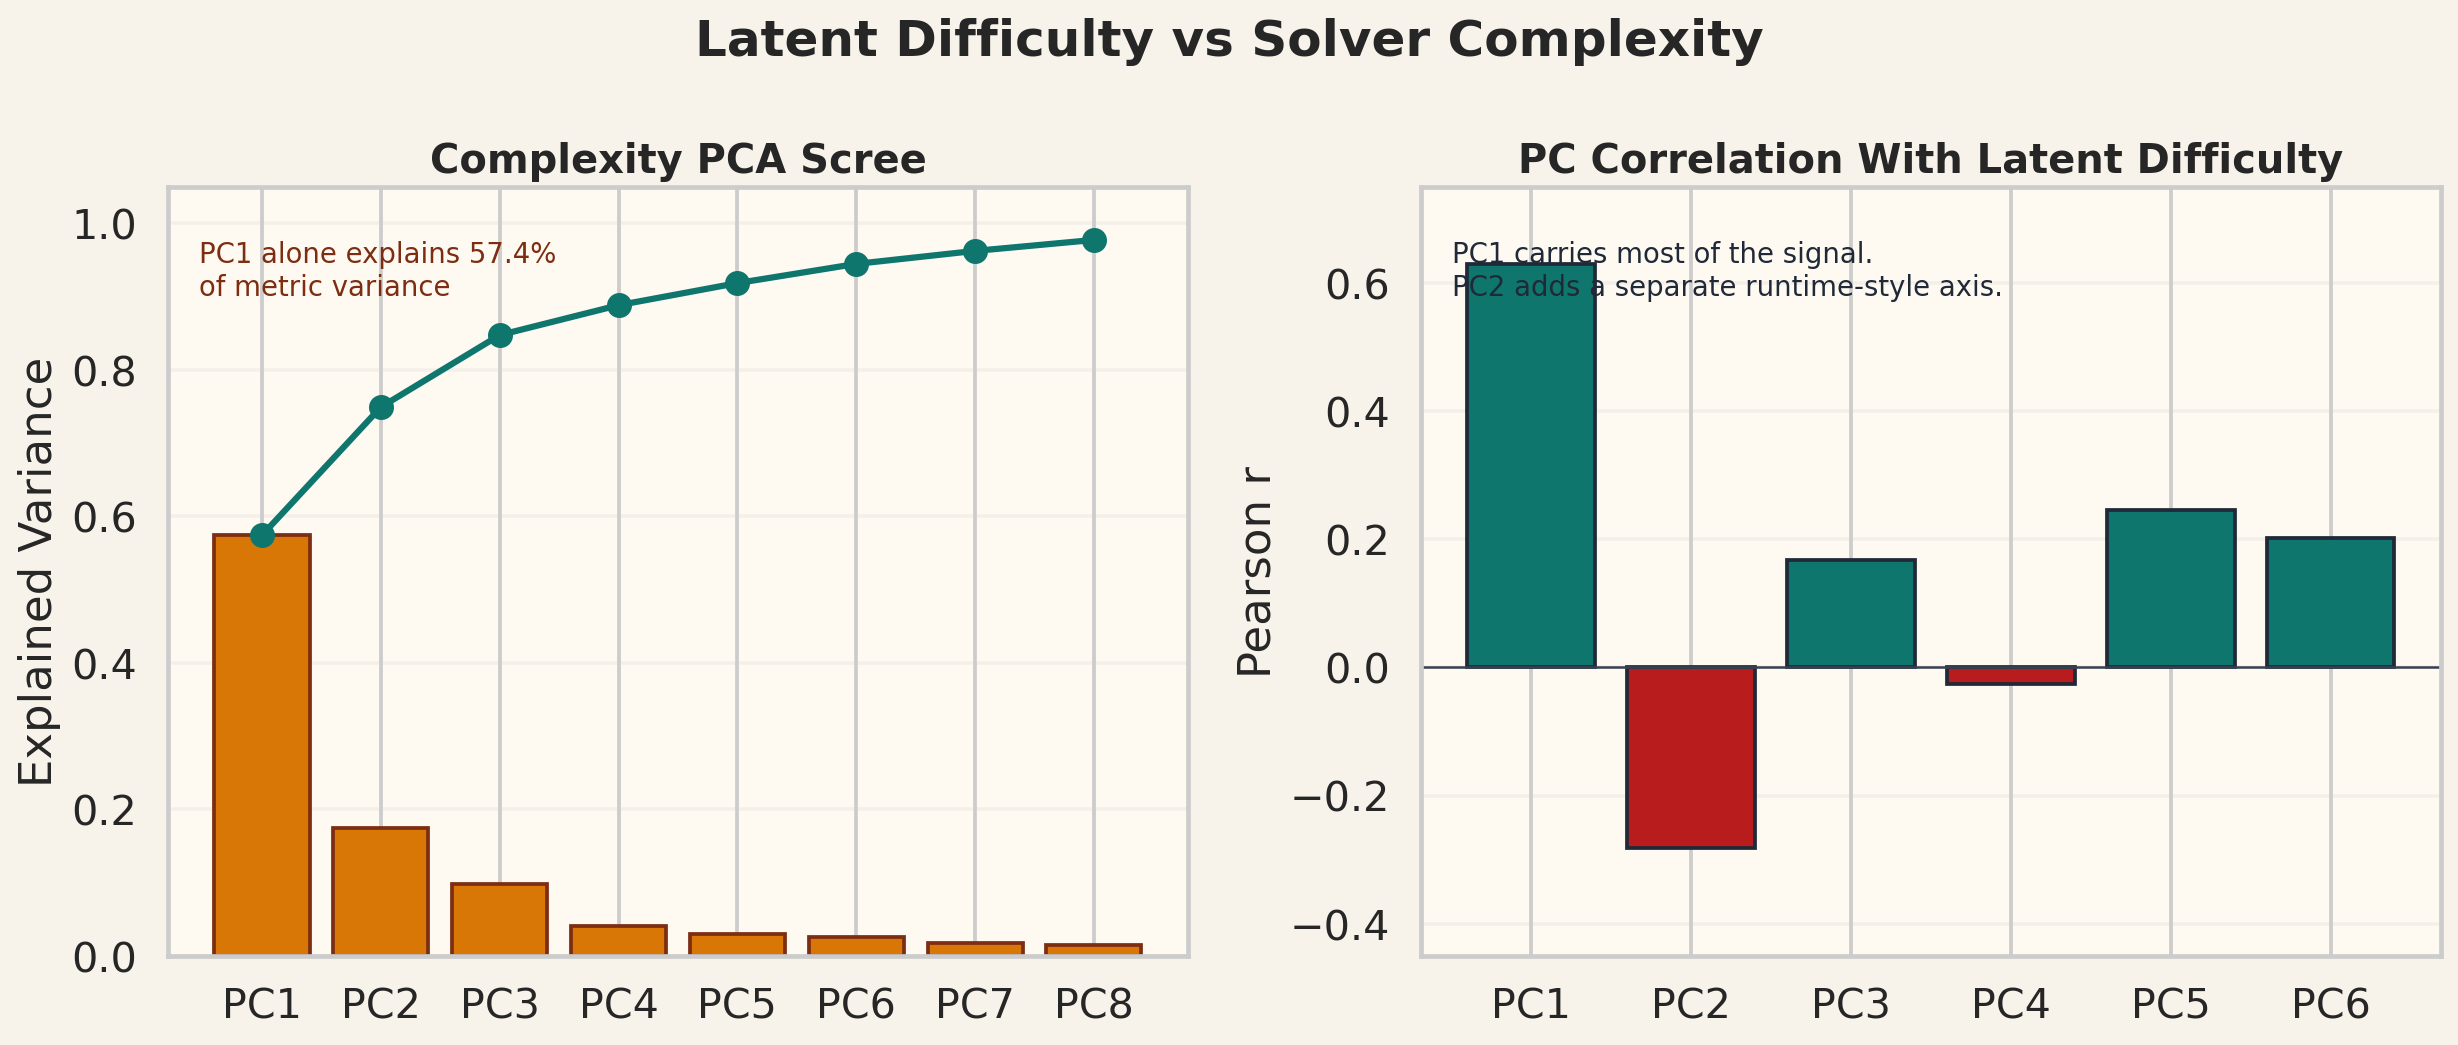
\includegraphics[width=0.9\textwidth]{chart_pca_overview.png}
    \caption{PCA overview of the validated solver-complexity panel. This figure matters because it shows that the complexity predictors are themselves organized into interpretable axes rather than arbitrary hand-picked metrics.}
\end{figure}

\begin{figure}[H]
    \centering
    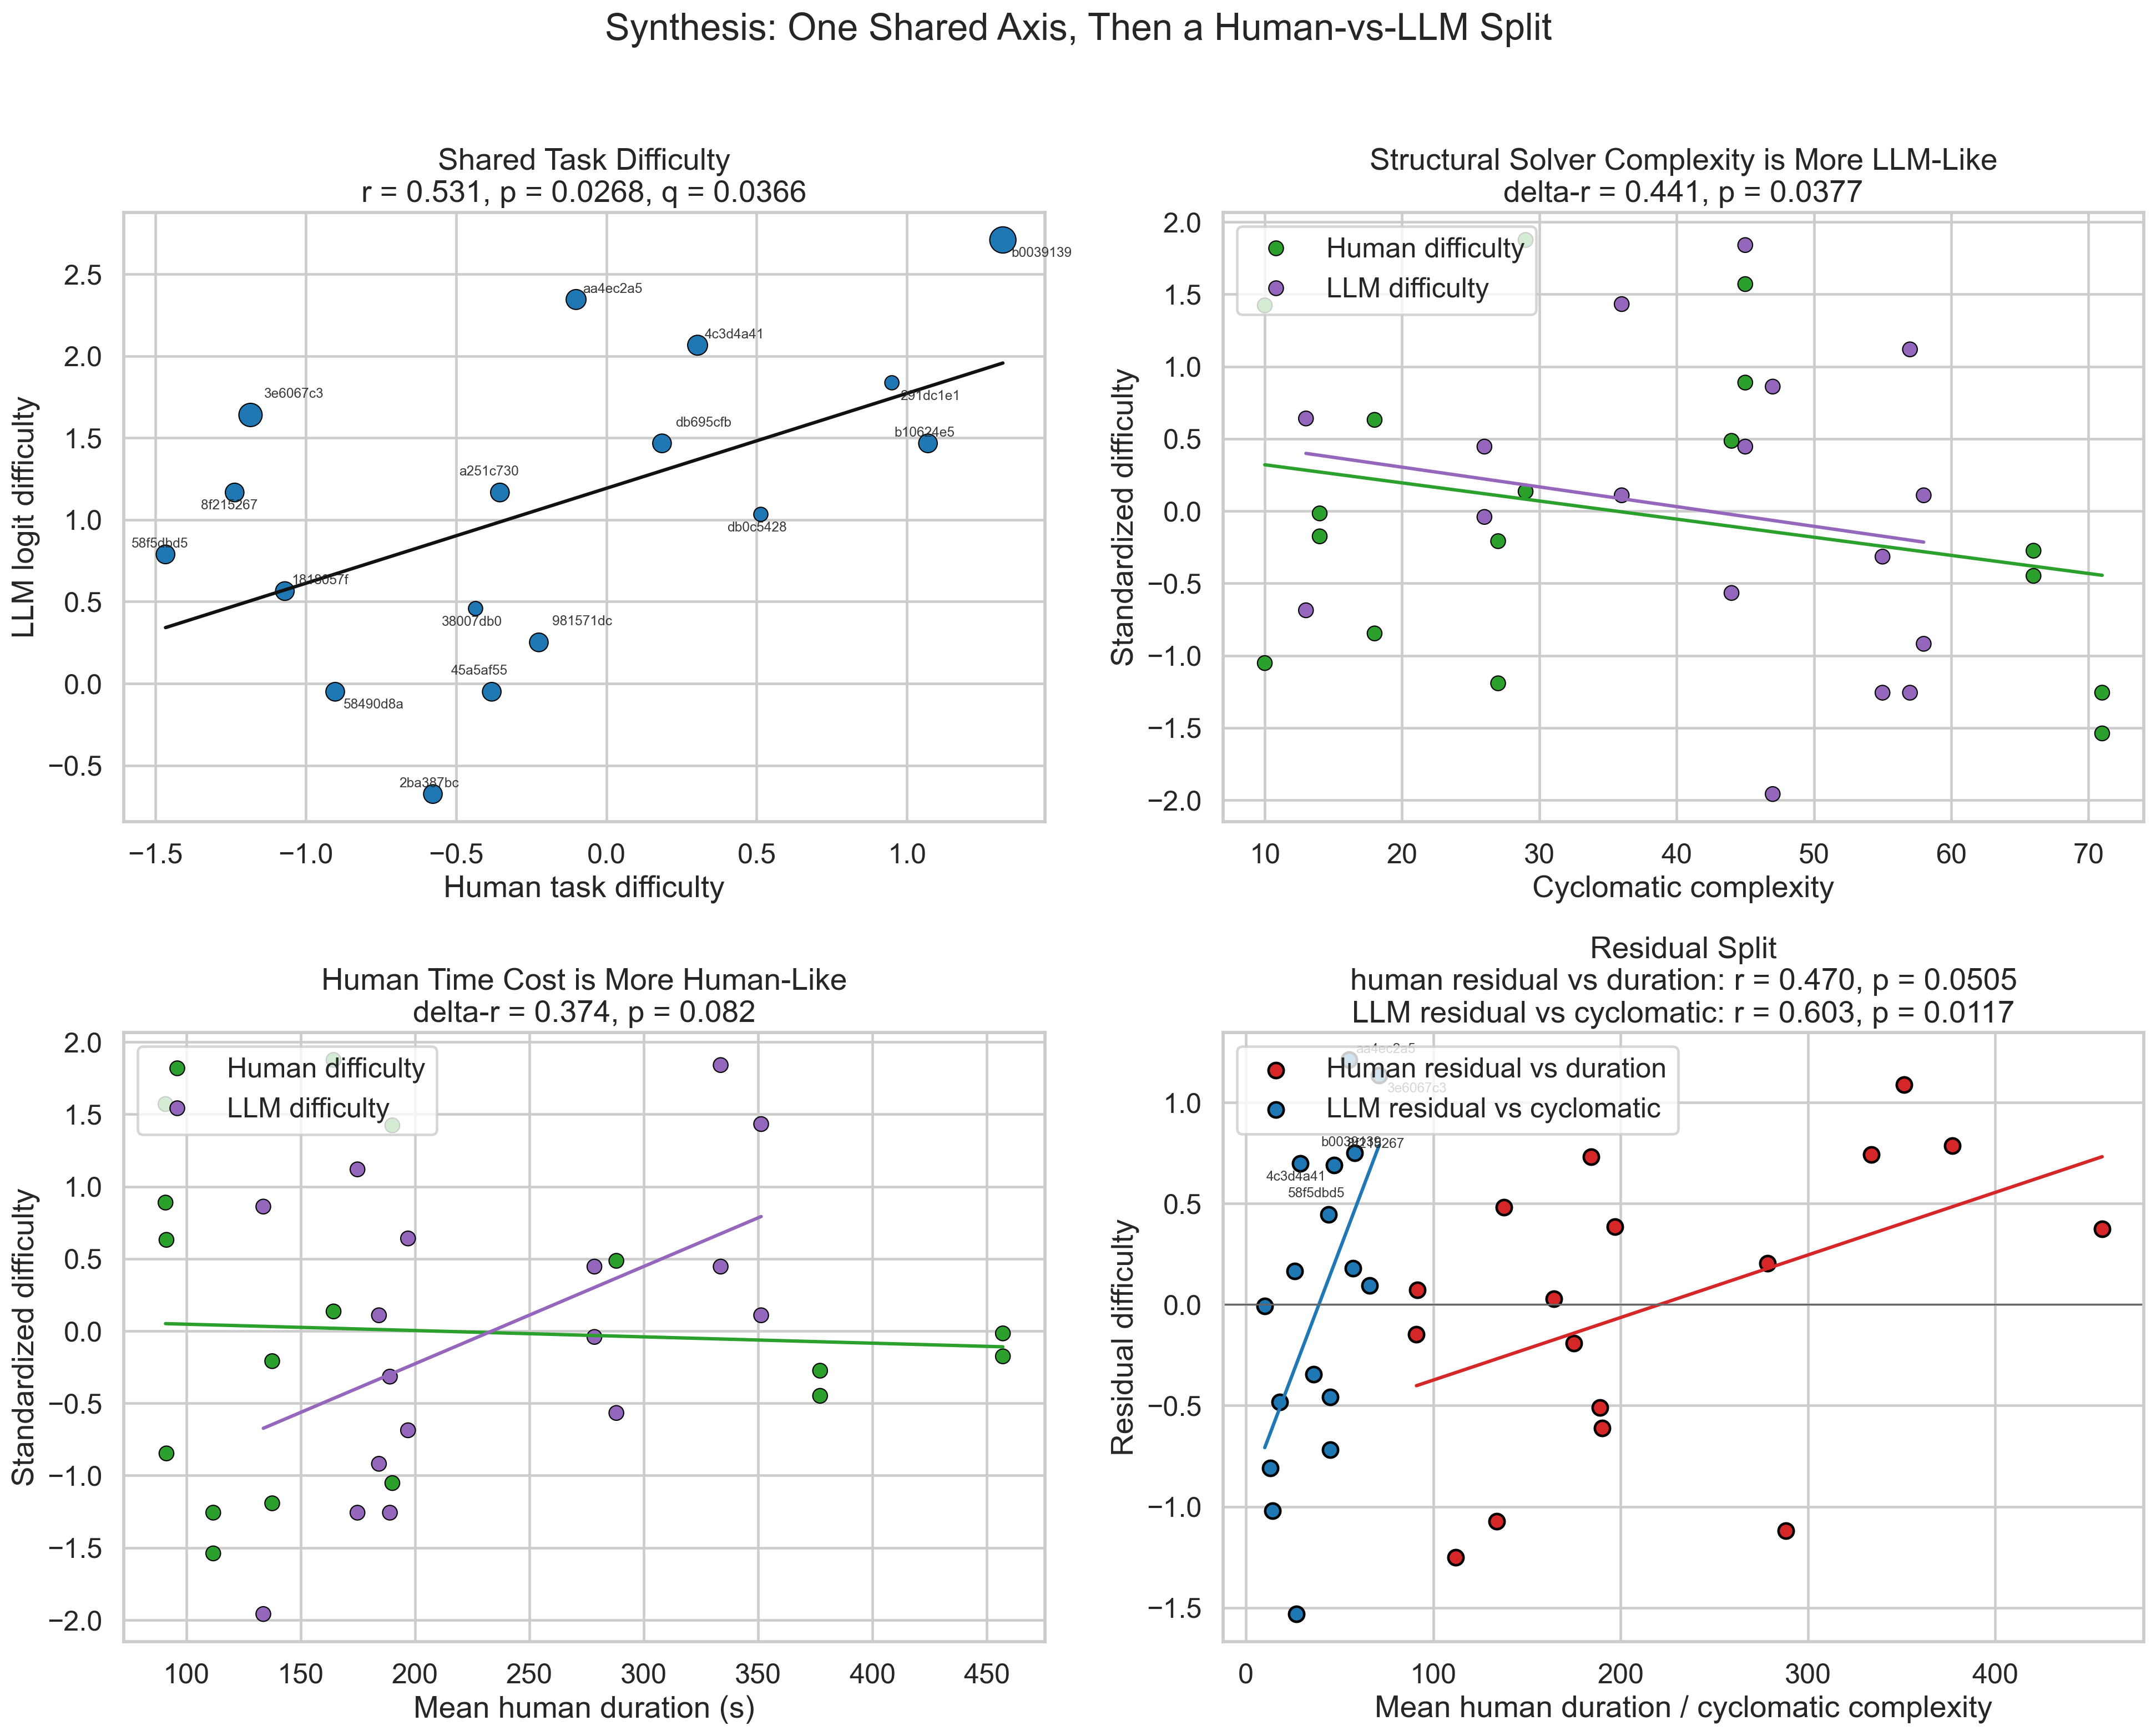
\includegraphics[width=\textwidth]{chart_synthesis_throughline.png}
    \caption{Through-line synthesis chart from the complexity package. The visual argument is the same as the statistical one: there is a shared human/LLM axis, followed by a split in what explains the residual burden.}
\end{figure}

\begin{figure}[H]
    \centering
    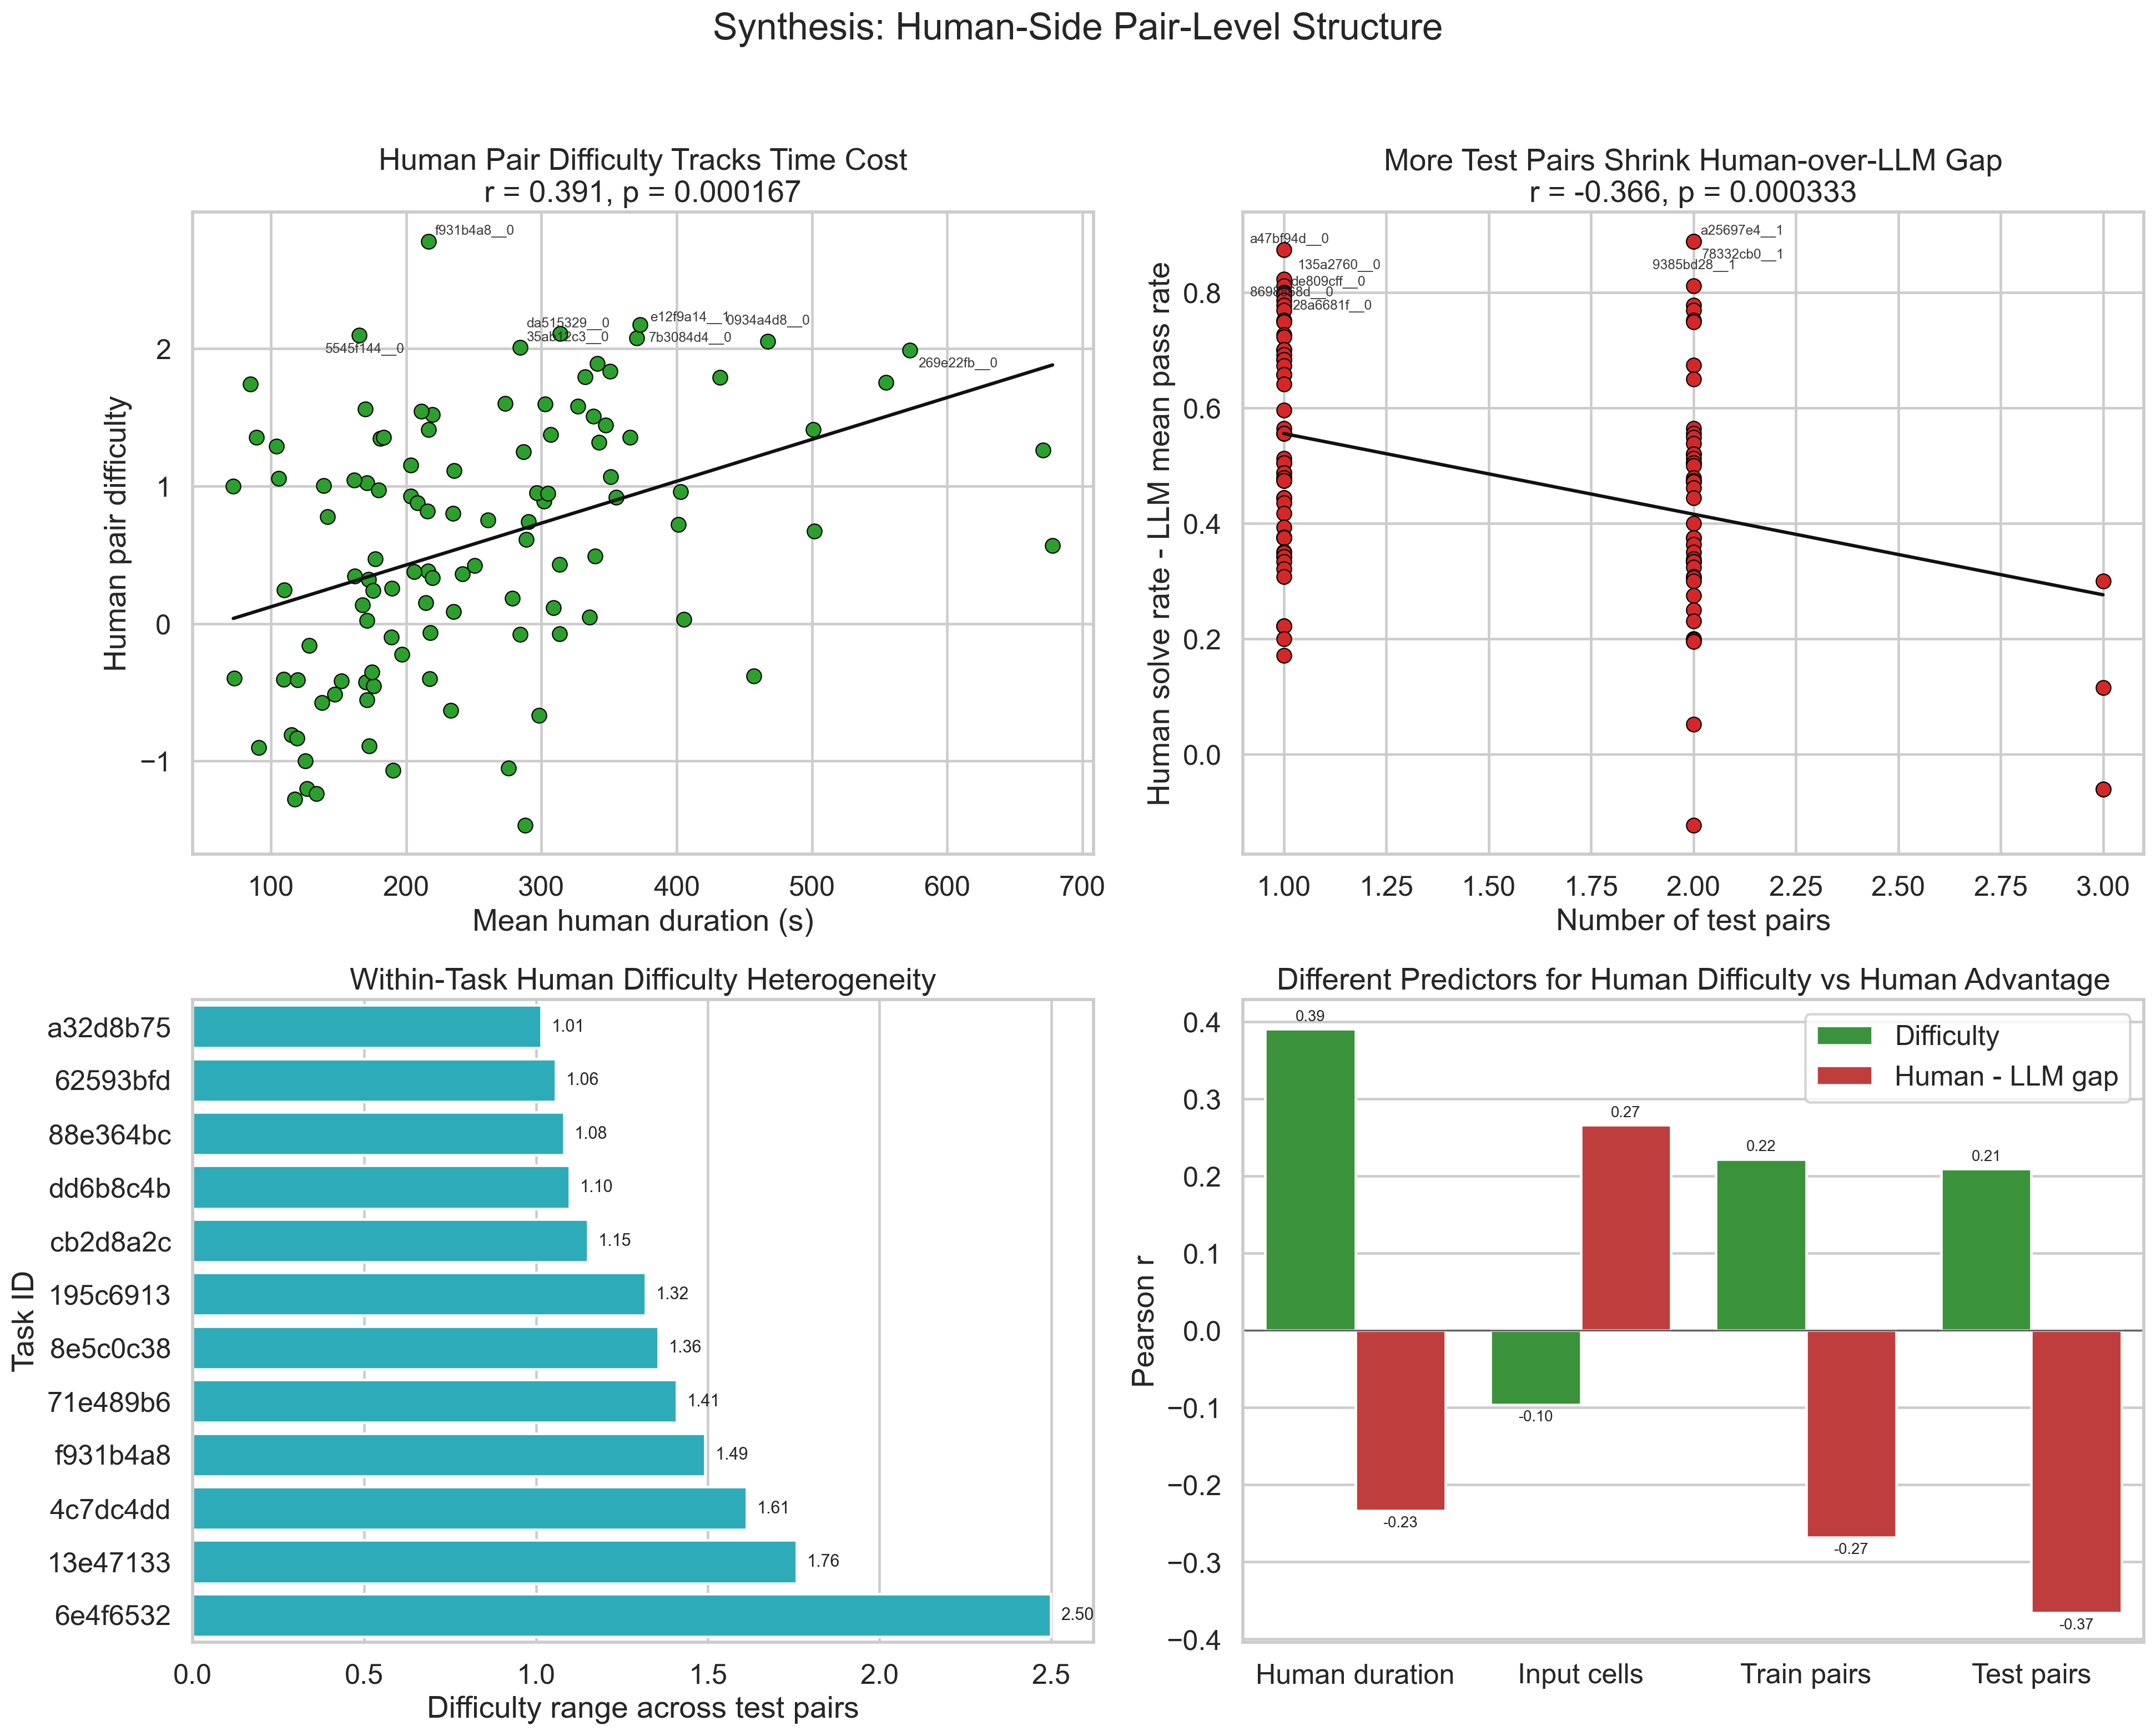
\includegraphics[width=\textwidth]{chart_synthesis_human_pair_level.png}
    \caption{Human-side pair-level structure from the complexity synthesis. Human burden is more time- and interaction-sensitive than a pure final-solver-size story would predict.}
\end{figure}

\begin{figure}[H]
    \centering
    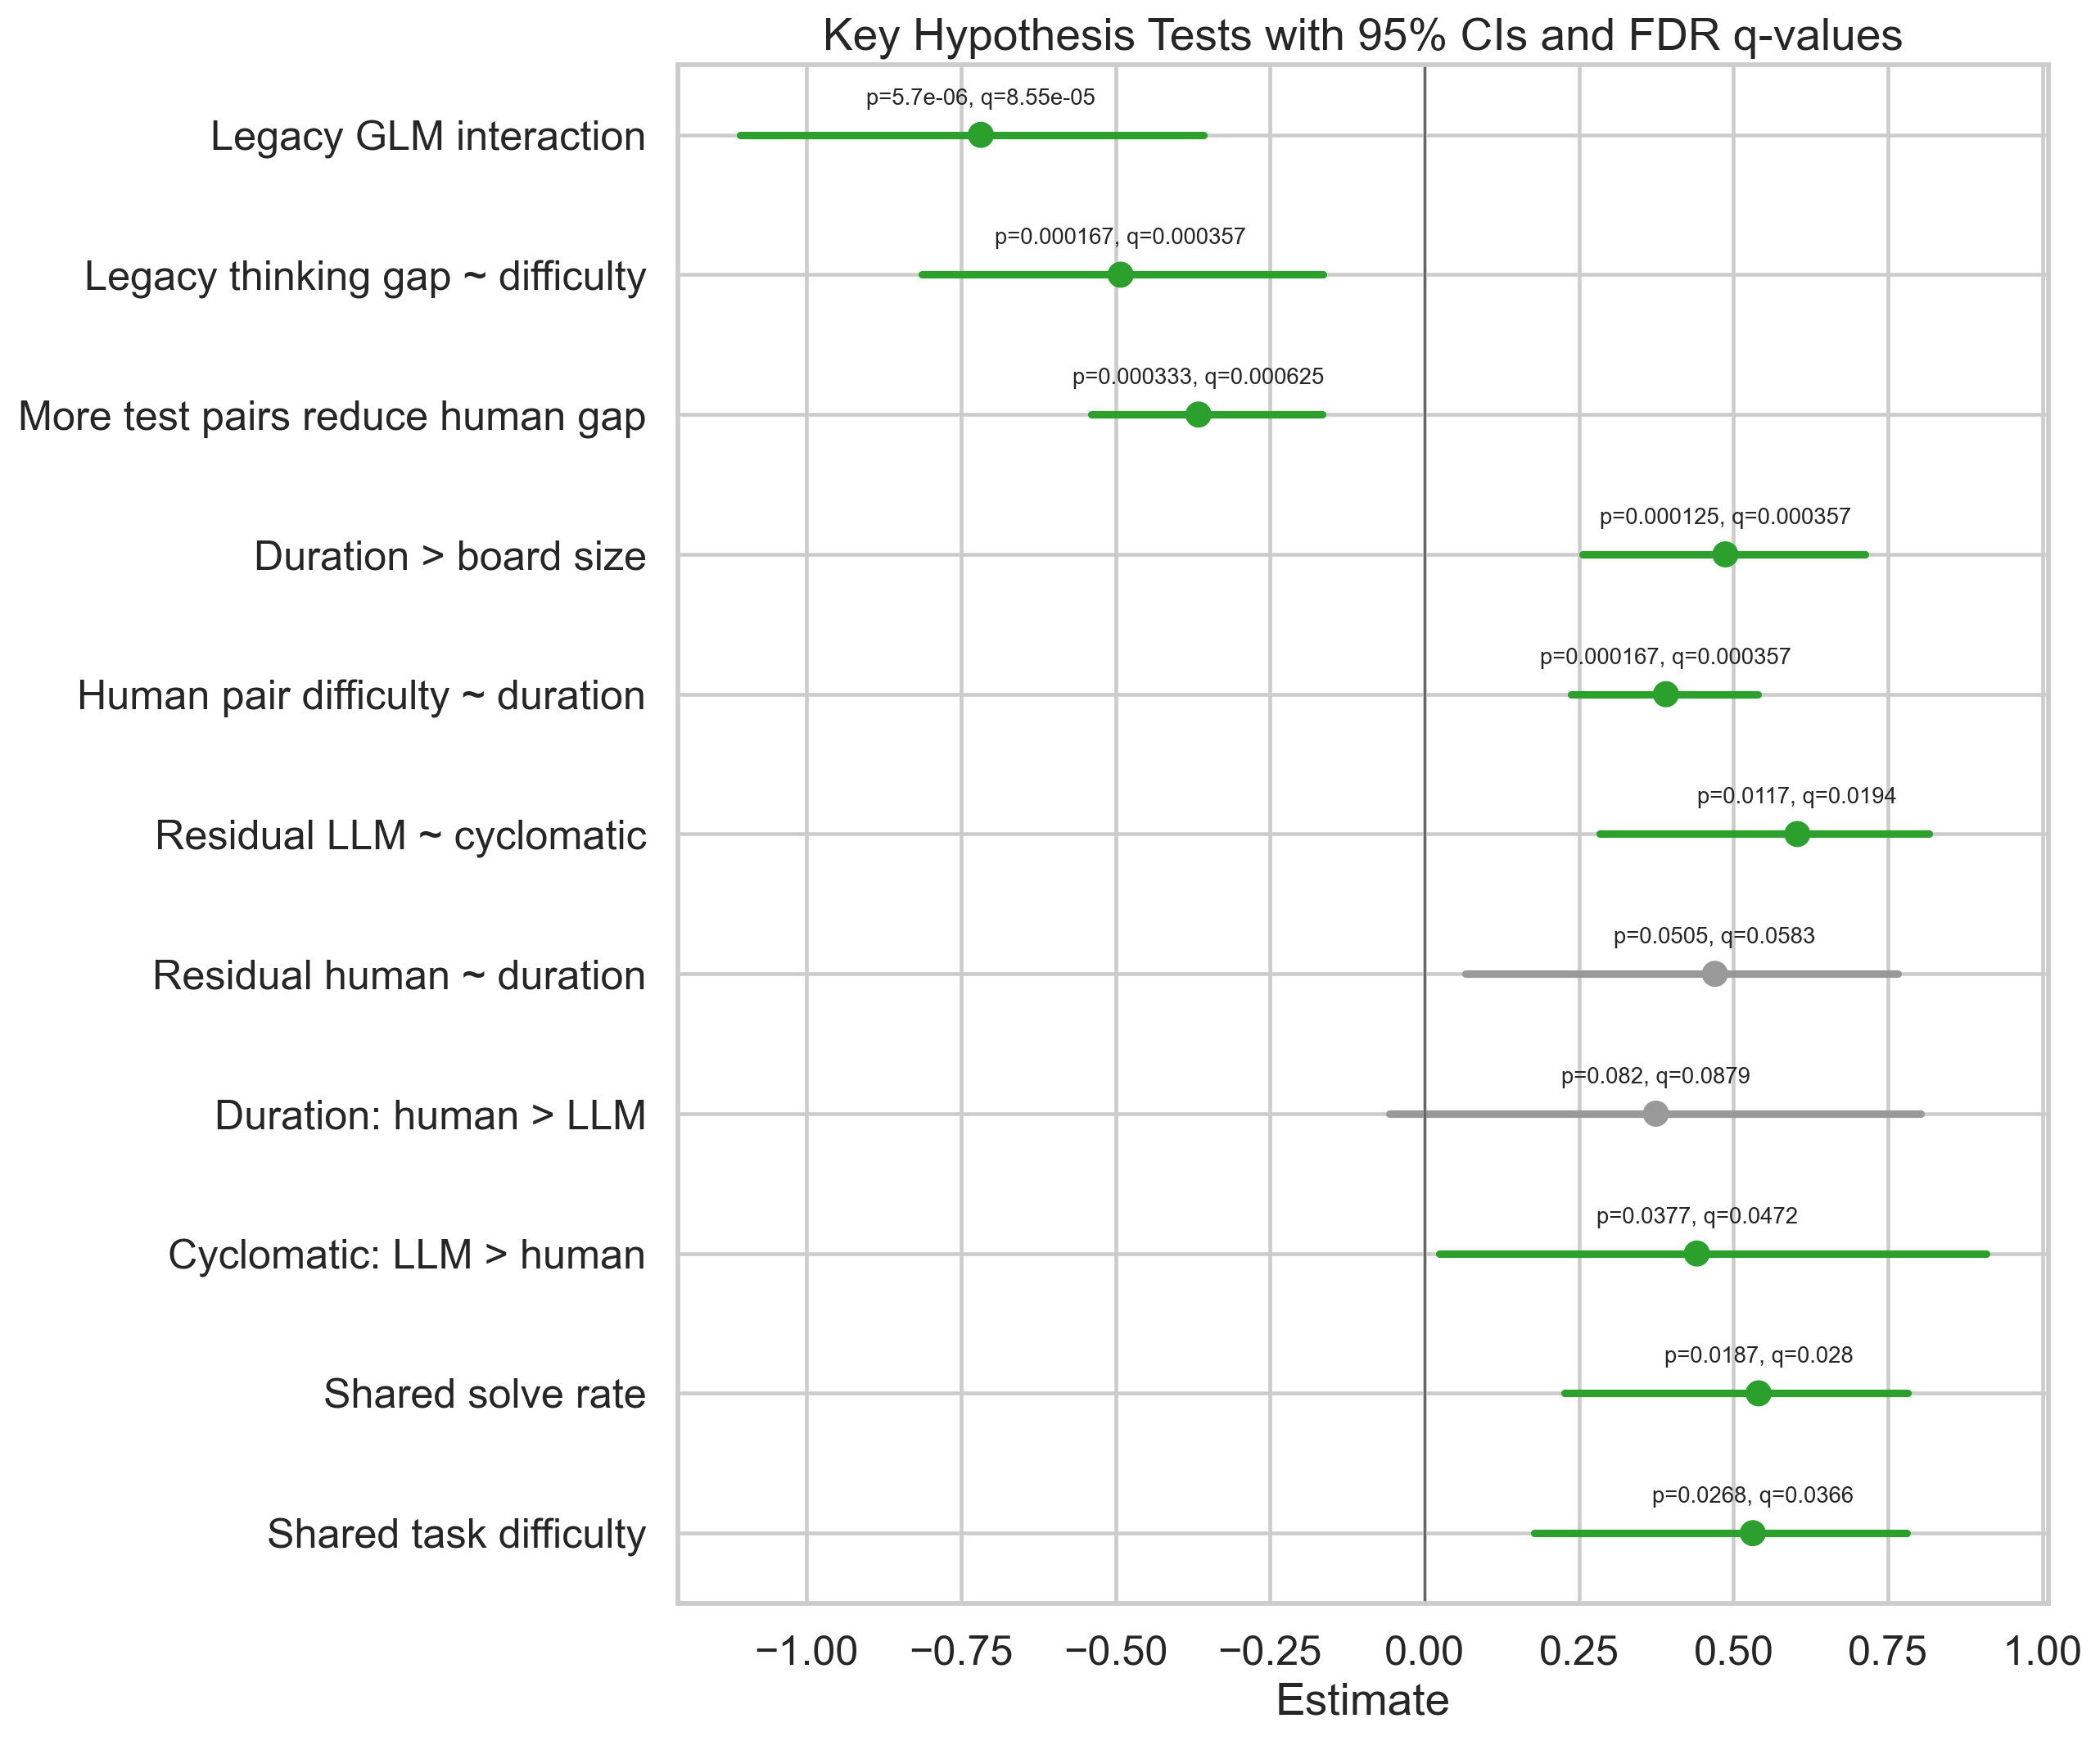
\includegraphics[width=0.92\textwidth]{chart_synthesis_stats_forest.png}
    \caption{Key hypothesis estimates with confidence intervals from the statistical audit. The most important surviving difference claim is that solver structure is more strongly linked to LLM difficulty than to human difficulty.}
\end{figure}

\subsection{Why this section matters for the rest of the paper}

This is the section that turns the repository from a pile of comparisons into an argument. The paper's main thesis is not just that humans and models overlap on ARC. It is that they overlap on one difficulty axis while loading differently on final-solver structure, time cost, and pair-level heterogeneity. That interpretation comes primarily from the solver-complexity line.

% ===== Cross-ARC Linkage and Efficiency =====
\section{Cross-ARC Linkage and Efficiency}

\subsection{Goal}

The goal of the cross-ARC and efficiency workstreams was to widen the context around the tiny fully matched overlap. Cross-ARC asks whether sparse human task estimates can be stabilized and linked across ARC-AGI-1 and ARC-AGI-2 without pretending the benchmarks are identical. Efficiency asks whether score, duration, cost, and effort tell a consistent story across humans, LLMs, and non-LLM systems.

\subsection{Data}

The cross-ARC package constructs three benchmark slices: an ARC-1 sidecar with 230 human-covered tasks, an ARC-2 eval slice with 115 matched human and LLM tasks, and an ARC-2 train-other slice with 97 tasks. The efficiency package aggregates 29 LLM model runs, 509 human sessions, 15 non-LLM rows, and 115 shared ARC-2 tasks for direct cross-source task-level comparison.

\subsection{Methods}

Cross-ARC uses latent task estimation, split-half stability comparisons, benchmark metadata, and common-model linkage between ARC-1 and ARC-2. Efficiency uses source-family rollups, task-level cross-source correlations, within-source efficiency gradients, cross-validated predictive models, and shared-task PCA. The common methodological idea is to widen the interpretive field without pretending that every source family lives on one perfectly commensurate scale.

\subsection{Experiment}

The cross-ARC line first asks whether latent task estimates are more stable than raw solve rates under sparse human coverage. It then asks how strongly human and LLM difficulty align on the widened ARC-1 and ARC-2 slices, and whether the main solver-structure asymmetry survives that wider linkage. The efficiency line then asks whether shared-task score alignment is accompanied by effort alignment, and whether simple geometry plus machine-side features can predict human outcomes.

\subsection{Results}

The first cross-ARC result is methodological but important: latent task estimates are more stable than raw solve rates in every benchmark slice. The latent-minus-raw gain is about 0.064 in the ARC-1 sidecar, about 0.068 in ARC-2 eval, and about 0.087 in ARC-2 train-other. The second result is that widened human-versus-LLM alignment is real but moderate: latent human difficulty correlates with LLM difficulty around $r = 0.309$ in ARC-1 sidecar and around $r = 0.355$ in ARC-2 eval.

The third result is that the main structure asymmetry still appears when the overlap is widened. On the direct ARC-2 eval revisit, cyclomatic complexity correlates about $r = 0.188$ with human difficulty and about $r = 0.600$ with LLM difficulty. That is directionally the same result as the main complexity paper, not a contradiction of it.

The efficiency package then adds a different kind of evidence. On the 115 shared ARC-2 tasks, human solve rate versus LLM mean score is about 0.440 Pearson and 0.428 Spearman. Human solve rate versus TRM best task score is near zero. Within source families, LLM performance rises strongly with thinking rank and duration, while human performance rises strongly with latent ability and falls with mean duration. The best cross-validated model for human solve rate is a geometry-plus-LLM-performance model, but human duration remains poorly predicted. That is a concise way of saying that score alignment is clearer than effort alignment.

\begin{table}[H]
\centering
\small
\caption{Widened human-versus-LLM alignment across the cross-ARC slices. The latent column is the one the paper treats as primary, but the raw and PC1 columns show that the effect is not an artifact of one estimator.}
\begin{tabular}{p{1.2in}p{0.8in}p{1.0in}p{1.0in}p{1.0in}}
\toprule
\textbf{Slice} & \textbf{$n$ tasks} & \textbf{Raw solve vs LLM} & \textbf{Latent vs LLM} & \textbf{PC1 vs LLM} \\
\midrule
ARC-1 sidecar & 230 & 0.297 & 0.309 & 0.362 \\
ARC-2 eval & 115 & 0.368 & 0.355 & 0.341 \\
\bottomrule
\end{tabular}
\end{table}

\begin{table}[H]
\centering
\small
\caption{Direct-overlap structure deltas in the widened revisit. Even on the small revisit slice, the same asymmetry reappears: solver structure is more LLM-linked than human-linked.}
\begin{tabular}{p{1.8in}p{0.6in}p{0.8in}p{0.8in}p{0.8in}}
\toprule
\textbf{Predictor} & \textbf{$n$} & \textbf{Human $r$} & \textbf{LLM $r$} & \textbf{$\Delta$} \\
\midrule
Cyclomatic complexity & 19 & 0.188 & 0.600 & 0.412 \\
Structure PC1 & 19 & 0.173 & 0.552 & 0.378 \\
\bottomrule
\end{tabular}
\end{table}

\begin{table}[H]
\centering
\scriptsize
\caption{Selected efficiency correlations. The table is organized to show within-source gradients first and shared-task cross-source gradients second.}
\begin{tabular}{p{2.6in}p{0.45in}p{0.7in}p{0.7in}}
\toprule
\textbf{Analysis} & \textbf{$n$} & \textbf{Pearson} & \textbf{Spearman} \\
\midrule
LLM performance vs thinking rank & 22 & 0.749 & 0.805 \\
Human performance vs ability & 509 & 0.878 & 0.873 \\
Human performance vs duration & 509 & -0.280 & -0.338 \\
Shared-task human vs LLM score & 115 & 0.440 & 0.428 \\
Shared-task human vs LLM duration & 115 & -0.284 & -0.332 \\
Shared-task human vs LLM cost & 115 & -0.311 & -0.357 \\
Shared-task human vs TRM score & 115 & 0.071 & 0.055 \\
Public-eval human vs average model & 110 & 0.402 & 0.454 \\
Public-eval human vs best single model & 110 & 0.276 & 0.276 \\
\bottomrule
\end{tabular}
\end{table}

\begin{figure}[H]
    \centering
    \includegraphics[width=0.92\textwidth]{human_llm_alignment.png}
    \caption{Cross-ARC human-versus-LLM alignment view. The widened ARC-1 and ARC-2 matches preserve the same basic story as the smaller direct overlaps: shared structure is real, but not complete.}
\end{figure}

\begin{figure}[H]
    \centering
    \includegraphics[width=0.82\textwidth]{solver_structure_cyclomatic.png}
    \caption{Cross-ARC solver-structure revisit. Even on the widened revisit slice, cyclomatic complexity tracks LLM difficulty much more strongly than human difficulty.}
\end{figure}

\begin{figure}[H]
    \centering
    \includegraphics[width=0.94\textwidth]{shared_task_latent_map.png}
    \caption{Shared-task latent map from the efficiency package. This view is useful because it ties the cross-ARC linkage work back to the concrete 115-task overlap used for score and effort comparisons.}
\end{figure}

\begin{figure}[H]
    \centering
    \includegraphics[width=0.96\textwidth]{task_correlation_heatmap.png}
    \caption{Task-correlation heatmap across shared-task metrics. The main pattern is that score-like variables cluster together more clearly than effort-like variables do across source families.}
\end{figure}

\begin{figure}[H]
    \centering
    \includegraphics[width=\textwidth]{source_tradeoff.png}
    \caption{Efficiency tradeoff view across source families. LLM gains are tied strongly to additional thinking and runtime; human performance varies much more with latent ability than with a machine-like cost signal.}
\end{figure}

\subsection{Why this section matters for the rest of the paper}

These packages do not replace the main complexity result; they widen and stress-test it. Cross-ARC shows that the sparse human data become more stable under latent estimation and that the shared human-versus-LLM axis survives beyond the tiny fully matched slice. Efficiency shows that score alignment does not imply common effort structure. Together they make the repo's final thesis harder to dismiss as a quirk of one tiny overlap table.

% ===== Architectural Synthesis =====
\section{Architectural Synthesis}

\subsection{Why the external literature belongs inside the same paper}

The repository does not only contain empirical comparison packages. It also contains a separate synthesis of four recent ARC solver papers: URM, TRM, VARC, and McGovern's test-time adaptation study. At first glance, that literature review might look like a side project. In practice, it may be the clearest mechanistic frame for the mixed empirical picture the repo keeps finding. The architecture section therefore should not be treated as optional context. It is the place where the full paper explains why the empirical divergence across humans, LLMs, and non-LLM systems might exist.

\subsection{What ARC demands from a solver}

The external synthesis starts from two simple but load-bearing facts about ARC itself. The sample budget is tiny: two to four demonstrations is not enough to fit a flexible learner from scratch. And evaluation is pixel-perfect: a single wrong cell fails the task. Together these constraints push successful systems toward strong priors, discrete hypothesis maintenance, and some kind of test-time refinement or selection loop. This matters because it links the external architecture papers back to the internal empirical results. If ARC inherently rewards structured iterative search under strong inductive bias, then it becomes more plausible that final solver structure would track model difficulty strongly and that some non-LLM systems would solve complementary items even before they look broadly human-like.

\subsection{The common loop}

The existing synthesis paper argues that these non-LLM architectures all converge on one computational loop. They encode the task with strong inductive bias, iteratively refine a hypothesis, decode a candidate answer, and select or marginalize across candidates at test time. The details differ. URM and TRM use recurrent or looped computation. VARC uses vision priors and test-time training. McGovern studies what survives when test-time adaptation is squeezed under strict compute limits. But the common pattern remains the same: strong priors plus structured test-time search.

\subsection{URM and the case for recurrent depth}

URM provides one of the clearest ablation stories in the external bundle. Under an equal compute multiplier, reallocating compute from non-shared depth toward recurrent weight-shared passes improves ARC-AGI-1 pass@1 from about 23.75\% to 40.0\%. The paper's interpretation is that iterative refinement is a better use of compute than simply adding more distinct layers for ARC-style reasoning. URM also reports that the nonlinear gated MLP path is load-bearing and that certain recurrence-training choices, such as truncated backpropagation through loops, matter substantially.

Why does that matter for the repo-wide story? Because it gives a mechanistic candidate for why ARC difficulty might look strongly structure-loaded to LLM-like systems. If successful solution requires repeated structured transformation of a latent hypothesis, then tasks with more branching, object bookkeeping, or nested logic should demand more iterative updates. That is very close to what the internal solver-complexity line is measuring.

\subsection{TRM and the latent scratchpad interpretation}

TRM arrives at a more interpretable version of the same broad idea. Instead of emphasizing recurrence mainly as efficient depth, TRM frames the hidden state as containing both a candidate answer and a reasoning scratchpad. The model is tiny, around 7M parameters, yet reaches roughly 45\% pass@1 on ARC-AGI-1 in the cited paper. Test-time augmentation is central rather than secondary, with about 1000 transformed views contributing to plurality voting.

This matters for the master paper because TRM illustrates both the promise and the current limits of non-LLM ARC progress. Architecturally, it is exactly the kind of system that might expose a more human-relevant inductive bias or search loop. Empirically, in the current repo it still does not align with human difficulty especially well on the primary ARC-2 overlap. The combined interpretation is not that TRM is uninteresting. It is that promising mechanism and current psychometric human-likeness are not the same thing.

\subsection{VARC and visual inductive bias}

VARC makes the boldest representational claim: ARC is primarily a vision problem rather than a language problem. Its core move is to treat ARC tasks as image-to-image transformations on a canvas with two-dimensional inductive bias. The paper's own ablations support this strongly. Replacing 2D rotary positional encoding with 1D positional encoding drops pass@2 from about 54.5\% to 51.0\%, and the broader package shows very large gains from test-time training, multi-view inference, and ensemble selection. In the reported chain, single-view no-TTT performance around 35.9\% grows to about 49.8\% with multi-view plus TTT, then to about 54.5\% at pass@2, and to about 60.4\% in the final ensemble.

For the repo-wide synthesis, VARC is important for two reasons. First, it shows that better inductive bias can matter as much as, or more than, raw parameter count for ARC. Second, it clarifies why multi-view and candidate-selection strategies might create complementary successes without yet producing a globally human-like psychometric profile. A system can have the right modality prior for some tasks and still place its wins on a different slice of the task distribution than humans do.

\subsection{McGovern and compute-limited adaptation}

McGovern's study is the most operationally grounded of the set because it asks what survives under ARC Prize style compute limits. The gap it highlights is severe: competition-time fine-tuning is roughly a 1/32 compute regime compared with unconstrained pretraining. A pretrained TRM fine-tuned for 12,500 steps reaches about 6.67\% on the semi-private tasks versus about 10\% for the fully pretrained version. That is a gap, but not a total collapse. The practical lesson is that pretraining plus limited adaptation can still be meaningful under strict budget.

The paper's most informative negative result is that fine-tuning only task embeddings while freezing the trunk yields near-zero performance. This cuts against a simple story in which the task token contains a soft executable program while the backbone merely interprets it. Instead, useful adaptation appears to require broader network updates. This again harmonizes with the internal repo picture: ARC-solving burden is not obviously localized in one tiny module. It appears distributed across the system's update dynamics and representational machinery.

\subsection{How the literature and repo evidence fit together}

The external literature and the internal empirical analyses fit together better than they might initially seem to. The complexity line says that final solver structure is especially explanatory for LLM difficulty. The human line says that human burden is more duration- and interaction-sensitive. The non-LLM line says that current structured solvers add complementary signal without yet matching the human profile broadly. The architecture papers say that strong priors, iterative refinement, and test-time candidate selection are the load-bearing mechanisms in current small-model ARC progress.

Taken together, those two bodies of evidence suggest a disciplined mechanistic interpretation. ARC seems to contain a shared abstraction burden plus source-specific execution burden. For current LLM-like systems, that burden is revealed strongly by the structure of a final successful solver. For humans, that solver structure only partly captures the burden because humans are also paying search, interaction, and pair-specific costs. For current non-LLM systems, the architecture papers imply that the important ingredients may already be present, but the psychometric comparisons suggest those ingredients have not yet produced broad human-like item ordering on the current overlap.

\subsection{What this section licenses and what it does not}

This external synthesis licenses a much stronger mechanistic hypothesis than the repo could support from psychometric tables alone: that a common loop of strong prior plus iterative refinement plus candidate selection may underlie recent small-model ARC progress. But it does not license the claim that these systems solve ARC the way humans do. The repo does not have human process traces rich enough to support that. The most responsible use of the architecture section is therefore explanatory and generative. It helps explain why the non-LLM systems may still matter despite weak human-alignment numbers, and it generates concrete next questions about invariance, iterative search, and the role of latent scratchpads or task adaptation.

% ===== Integrated Discussion =====
\section{Integrated Discussion}

\subsection{What is strongest in the repository}

The full repository does not support every attractive story equally well. Its strongest supported thesis has three parts. First, there is a real shared difficulty axis across humans and machine systems on ARC. Second, validated final solver structure is one of the strongest explanatory variables for LLM difficulty in the entire repo. Third, human burden is not captured by that same structure to the same degree and instead looks more tied to time cost, search burden, and pair-level heterogeneity.

\subsection{What should be treated as central versus secondary}

If the paper is trying to be intellectually honest, it should rank its findings rather than narrate them all at the same volume. The central retained claims are: ARC looks psychometrically clean on the LLM side; sparse human ARC data are usable once reliability is estimated explicitly; human-versus-average-model alignment is real but bounded by human split-half reliability; validated solver structure predicts LLM difficulty strongly; the solver-structure link is significantly stronger for LLM difficulty than for human difficulty; and current non-LLM systems do not reproduce the human difficulty profile as well as the LLM consensus does. Those are the pieces the repo keeps recovering from multiple directions.

Secondary but still worthwhile claims include the closeness augmentation result, which suggests softer output similarity adds human-relevant signal for duration and latent ease; the pooled cross-ARC extension, which supports the main asymmetry on a wider benchmark footprint; and the non-LLM ``middle'' pattern in the complexity panel, which is suggestive but underpowered. The paper should treat these as useful amplifiers and qualifiers, not as the main pillars of the argument.

\subsection{How the non-LLM result should be narrated}

The non-LLM section is likely to be the hardest part of the final paper to get right rhetorically. It will be tempting either to bury it because it is weaker than hoped or to oversell its complementarity because the raw psychometric result is disappointing. Neither move would help. The most credible framing is this: current non-LLM systems are not yet the clean human-like alternative to the LLM consensus on ARC, but they are also not vacuous. They contribute complementary successes, expose a split between benchmark score and human-like item placement, and converge architecturally on a loop that may be important even where the current psychometric results remain modest.

\subsection{What the paper should explicitly flag as pressure points}

Several pressure points deserve explicit flagging in the manuscript rather than quiet footnotes. The first is the tiny fully matched human-plus-LLM-plus-non-LLM-plus-complexity overlap, which is effectively an ARC-2 comparison on 17 independent tasks. The second is the task-level versus pair-level mismatch: final solver files are task objects, but human burden often varies by pair. The third is the sampling character of the human dataset, which is sparse, opportunistic, and not a balanced exam design. The fourth is benchmark drift between ARC-1 and ARC-2, including the fact that the six shared eval IDs preserve test examples but change training examples. The fifth is that final approved solver size is not minimal solver size, still less human conceptual complexity.

There is also a more subtle pressure point: exact-match success is both the right leaderboard metric and a lossy behavioral summary. The solution-closeness addenda show that softer metrics do carry some residual signal, especially for human time cost, but they do not overturn the exact-match complexity story. The paper should say this clearly, because otherwise readers may assume either that binary scoring is the whole truth or that any soft metric automatically invalidates it. Neither reading is right.

\subsection{What the paper should not claim}

The manuscript should avoid at least three overclaims. It should not say that current LLMs and humans solve ARC for the same reasons. The human-versus-LLM complexity asymmetry is direct evidence against that. It should not say that current non-LLM systems are broadly more human-like than LLMs on the available psychometric evidence. They are not. And it should not keep the original thinking-advantage result as a clean flagship claim. After label verification and floor-sensitive checks, that result is better described as an audited lead that did not hold up cleanly.

\subsection{What future work would actually matter}

The future-work section should not devolve into generic calls for more data. The repository already points to the highest-value next steps: increase the fully matched overlap, make the task-level versus pair-level distinction explicit across the manuscript, carry the strongest closeness sensitivity analyses forward without displacing the main binary complexity result, expand cross-ARC linkage carefully, and add a small number of high-yield figures that visualize the decomposition story directly.

More specifically, the next empirical milestone would be to obtain a larger human benchmark with richer pair-level and response-grid logging so that solver structure, exact correctness, wrong-answer closeness, and duration can all be modeled on the same tasks. On the machine side, the most valuable next step is probably not more leaderboard chasing. It is to test whether the architectural loop suggested by URM, TRM, VARC, and McGovern can be made to yield a more human-like item profile, or whether those systems will continue to improve score while drifting away from the human ordering the way TRM seems to in the current repo.

\subsection{What this first full-paper draft is actually for}

As a first full-paper draft, the main job of this manuscript is not to finish every figure or settle every caveat. It is to make the repository legible as one coherent scientific argument. The argument it currently supports is strong enough to be worth taking seriously and narrow enough to be scrutinized. ARC contains a real shared difficulty axis across humans and machine systems, but it does not impose identical burden on all of them. LLM difficulty is strongly linked to the structure of validated successful solvers. Human difficulty is linked more weakly to that structure and more strongly to time, search, and pair heterogeneity. Current non-LLM systems remain the most promising architectural alternative and the weakest psychometric match. That is a sufficiently sharp thesis to organize a much larger final manuscript around.

% ===== Repository Coverage Appendix =====
\appendix
\section{Repository Coverage Appendix}

\subsection{Why include a coverage appendix}

One risk in any repository-scale paper is that the narrative becomes cleaner than the evidence base that produced it. This appendix is included to reduce that risk. It makes explicit which major folders and local papers were absorbed into the master draft, what role they play, and whether their main claims are being treated as central, secondary, or downgraded. In other words, it is a compact bridge between the repo as a working analysis environment and the paper as a narrative artifact.

\subsection{Workstream-to-manuscript mapping}

\begin{table}[t]
\centering
\small
\caption{Primary repo workstreams and how they enter the master paper.}
\begin{tabular}{p{1.5in}p{1.9in}p{2.4in}}
\toprule
\textbf{Workstream} & \textbf{Main local materials} & \textbf{Role in the master paper} \\
\midrule
LLM psychometrics & ARC psychometric paper, export-package findings manifest, benchmark-manifold note & Establishes the clean machine-side difficulty axis and broader general-factor context \\
Human testing & Human psychometric report, public tables, split-half checks & Establishes sparse but usable human difficulty structure and reliability context \\
Human-model alignment addendum & Creme-style synthesis and gap tables & Calibrates what human-versus-model alignment means relative to human-versus-human alignment \\
Non-LLM psychometrics & Main psychometric report, hypothesis synthesis, threshold and feature tables & Shows that current non-LLM systems are weaker than hoped as human-profile matches but still partly complementary \\
Solver complexity & Complexity master paper, approved LLM report, statistical audit, human addenda, closeness analyses & Supplies the central integrative finding that solver structure is more LLM-linked than human-linked \\
Cross-ARC linkage & Cross-benchmark report, latent split-half summary, pooled structure tables & Widens the matched human/LLM context and stabilizes sparse human estimates \\
Efficiency & Efficiency report, shared-task correlations, within-source tradeoff tables & Characterizes how performance, duration, cost, and effort differ across source families \\
Architectural synthesis & URM, TRM, VARC, and McGovern synthesis paper & Provides the mechanistic explanation for why complementary non-LLM signal might exist despite weak current human-alignment numbers \\
\bottomrule
\end{tabular}
\end{table}

\subsection{Claim status ledger}

\begin{table}[t]
\centering
\small
\caption{High-level status of the main claim families carried forward from the repo.}
\begin{tabular}{p{2.0in}p{1.0in}p{2.8in}}
\toprule
\textbf{Claim family} & \textbf{Status} & \textbf{Reason for current treatment} \\
\midrule
ARC is strongly one-factor dominated on the LLM side & Retained strong & Supported by response-matrix structure, PCA, scalability, and broader benchmark comparisons \\
Sparse human ARC data are psychometrically usable & Retained strong & Supported by held-in diagnostics, split-half context, and latent-over-raw stability gains \\
Human versus average-model alignment is real & Retained strong & Correlation lands near the center of the human split-half distribution \\
Current non-LLM systems are broadly as human-like as the LLM consensus & Rejected & Primary overlap results do not support it \\
Current non-LLM systems add some complementary signal & Retained secondary & Supported by rescued human-easy and LLM-hard items and training-trajectory differences \\
Validated solver structure predicts LLM difficulty strongly & Retained strong & Recovered across multiple difficulty summaries and complexity metrics \\
Solver structure predicts human difficulty equally strongly & Rejected & Best supported difference claim in the repo argues the opposite \\
Latent task estimates are more stable than raw human task means & Retained strong & Supported across ARC-1 sidecar, ARC-2 eval, and ARC-2 train-other slices \\
Thinking advantage declines cleanly with item difficulty & Downgraded & Strong under legacy labels, weak after label audit and floor-sensitive checks \\
Soft output-closeness metrics overturn the exact-match story & Rejected & Softer metrics help as additive residual predictors, not as replacements for the main exact-match result \\
Non-LLM complexity sits cleanly between human and LLM complexity & Suggestive & Descriptively plausible but underpowered on the shared $n = 17$ ARC-2 tasks \\
\bottomrule
\end{tabular}
\end{table}

\subsection{What remains outside the current draft}

The current draft now carries the main figure and table spine from each empirical workstream, but it is still not the last editorial pass. The clearest remaining upgrades are to prune any redundant summary phrasing that survived the earlier scaffold stage, promote a small number of appendix-grade tables into canonical camera-ready forms, and decide which visuals are truly indispensable for a submission version versus this repository-scale synthesis version. A separate limitations section would also still help by gathering the benchmark-fragility issues that are currently distributed across methods and discussion. So this draft is no longer merely a scaffold, but it is still one revision short of a polished final manuscript.

% ===== Selected Result Tables Appendix =====
\section{Selected Result Tables Appendix}

\subsection{Why include detailed result tables}

The main text now carries the core figures and headline tables from each workstream, but a repo-scale paper also benefits from a second layer of detail that readers can inspect without reopening every local CSV. This appendix collects a few of the highest-yield exported tables in a compact format. The purpose is not to replace the narrative sections. It is to make the manuscript visibly closer to the underlying repository outputs.

\subsection{Extended LLM leaderboard excerpt}

\begin{table}[H]
\centering
\scriptsize
\caption{Extended leaderboard excerpt from the main LLM psychometric package. The appendix keeps a longer cut than the main text so the strength and steepness of the frontier ordering are visible in one place.}
\begin{tabular}{p{2.45in}p{0.8in}p{0.8in}p{0.8in}}
\toprule
\textbf{Model} & \textbf{Type} & \textbf{ARC-1} & \textbf{ARC-2} \\
\midrule
Gemini 3 Deep Think Preview & Thinking & 96.0\% & 32.5\% \\
Gemini 3 Pro Preview & Thinking & 85.5\% & 17.5\% \\
GPT-5 Pro (2025-10-06) & Thinking & 77.2\% & 8.3\% \\
GPT-5.1 Thinking High & Thinking & 72.3\% & 8.3\% \\
Claude Sonnet 4.5 Thinking 32k & Thinking & 69.4\% & 7.5\% \\
GPT-5.1 Thinking Medium & Thinking & 65.3\% & 5.0\% \\
Claude Sonnet 4.5 Thinking 16k & Thinking & 59.7\% & 4.2\% \\
Claude Haiku 4.5 Thinking 32k & Thinking & 59.4\% & 3.3\% \\
Grok 4 Fast Reasoning & Thinking & 50.0\% & 3.3\% \\
Claude Sonnet 4.5 Thinking 8k & Thinking & 49.2\% & 4.2\% \\
Claude Haiku 4.5 Thinking 16k & Thinking & 44.4\% & 1.7\% \\
GPT-5.1 Thinking Low & Thinking & 37.4\% & 0.8\% \\
\bottomrule
\end{tabular}
\end{table}

\subsection{Non-LLM threshold-sensitivity ledger}

{\scriptsize
\begin{longtable}{p{0.5in}p{0.5in}p{2.25in}p{0.7in}p{0.7in}}
\caption{Detailed threshold-sensitivity ledger for the selected ARC-2 overlap profiles. These rows are taken directly from the threshold-sensitivity export that underlies the condensed main-text table.} \\
\toprule
\textbf{Min attempts} & \textbf{$n$} & \textbf{System} & \textbf{Pair acc.} & \textbf{Human $r$} \\
\midrule
\endfirsthead
\multicolumn{5}{l}{\small\itshape Non-LLM threshold-sensitivity ledger (continued)} \\
\toprule
\textbf{Min attempts} & \textbf{$n$} & \textbf{System} & \textbf{Pair acc.} & \textbf{Human $r$} \\
\midrule
\endhead
2 & 161 & LLM average & 0.109 & 0.345 \\
2 & 161 & GPT-5.2 xhigh & 0.491 & 0.256 \\
2 & 161 & Claude Opus 16k & 0.174 & 0.348 \\
2 & 161 & TRM 651522 pass@2 & 0.099 & 0.090 \\
2 & 161 & TRM 361957 pass@2 & 0.050 & 0.164 \\
2 & 161 & VARC ARC-2 ViT pass@2 & 0.043 & 0.091 \\
3 & 159 & LLM average & 0.109 & 0.351 \\
3 & 159 & GPT-5.2 xhigh & 0.484 & 0.242 \\
3 & 159 & Claude Opus 16k & 0.176 & 0.362 \\
3 & 159 & TRM 651522 pass@2 & 0.101 & 0.098 \\
3 & 159 & TRM 361957 pass@2 & 0.050 & 0.171 \\
3 & 159 & VARC ARC-2 ViT pass@2 & 0.044 & 0.096 \\
5 & 129 & LLM average & 0.105 & 0.367 \\
5 & 129 & GPT-5.2 xhigh & 0.481 & 0.231 \\
5 & 129 & Claude Opus 16k & 0.163 & 0.403 \\
5 & 129 & TRM 651522 pass@2 & 0.093 & 0.095 \\
5 & 129 & TRM 361957 pass@2 & 0.039 & 0.199 \\
5 & 129 & VARC ARC-2 ViT pass@2 & 0.039 & 0.142 \\
8 & 110 & LLM average & 0.108 & 0.402 \\
8 & 110 & GPT-5.2 xhigh & 0.491 & 0.276 \\
8 & 110 & Claude Opus 16k & 0.164 & 0.439 \\
8 & 110 & TRM 651522 pass@2 & 0.109 & 0.113 \\
8 & 110 & TRM 361957 pass@2 & 0.045 & 0.214 \\
8 & 110 & VARC ARC-2 ViT pass@2 & 0.036 & 0.158 \\
\bottomrule
\end{longtable}
}

\subsection{Solver-complexity audit excerpt}

{\scriptsize
\begin{longtable}{p{0.5in}p{1.15in}p{0.85in}p{0.85in}p{0.75in}}
\caption{Selected rows from the solver-complexity hypothesis ledger. Claim IDs and families are preserved from the CSV so the appendix stays traceable to the audit exports.} \\
\toprule
\textbf{ID} & \textbf{Family} & \textbf{Estimate} & \textbf{BH $q$} & \textbf{FDR kept} \\
\midrule
\endfirsthead
\multicolumn{5}{l}{\small\itshape Solver-complexity audit excerpt (continued)} \\
\toprule
\textbf{ID} & \textbf{Family} & \textbf{Estimate} & \textbf{BH $q$} & \textbf{FDR kept} \\
\midrule
\endhead
S1 & shared\_alignment & 0.531 & 0.0366 & yes \\
S2 & shared\_alignment & 0.541 & 0.0280 & yes \\
S3 & llm\_internal\_consistency & 0.991 & 0.0004 & yes \\
S4 & llm\_internal\_consistency & 0.970 & 0.0004 & yes \\
D1 & difference\_claims & 0.441 & 0.0472 & yes \\
D2 & difference\_claims & 0.374 & 0.0879 & no \\
D4 & difference\_claims & 0.603 & 0.0194 & yes \\
H1 & human\_pair\_level & 0.391 & 0.0004 & yes \\
H3 & human\_pair\_level & 0.487 & 0.0004 & yes \\
H4 & human\_pair\_level & -0.366 & 0.0006 & yes \\
H5 & human\_pair\_level & 0.749 & 0.0004 & yes \\
T1 & thinking\_advantage & -0.492 & 0.0004 & yes \\
T2 & thinking\_advantage & -0.718 & 0.0001 & yes \\
\bottomrule
\end{longtable}
}

\subsection{Efficiency correlation ledger}

{\scriptsize
\begin{longtable}{p{2.8in}p{0.45in}p{0.7in}p{0.7in}}
\caption{Selected correlations from the efficiency package. The table is intentionally more complete than the main-text version so the performance, duration, cost, and effort relations can be inspected directly.} \\
\toprule
\textbf{Analysis} & \textbf{$n$} & \textbf{Pearson} & \textbf{Spearman} \\
\midrule
\endfirsthead
\multicolumn{4}{l}{\small\itshape Efficiency correlation ledger (continued)} \\
\toprule
\textbf{Analysis} & \textbf{$n$} & \textbf{Pearson} & \textbf{Spearman} \\
\midrule
\endhead
LLM performance vs thinking rank & 22 & 0.749 & 0.805 \\
LLM duration vs thinking rank & 22 & 0.609 & 0.815 \\
LLM performance vs duration & 29 & 0.387 & 0.672 \\
LLM duration vs cost & 29 & 0.698 & 0.670 \\
Human performance vs ability & 509 & 0.878 & 0.873 \\
Human performance vs duration & 509 & -0.280 & -0.338 \\
Human performance vs outfit & 509 & -0.458 & -0.691 \\
Shared-task human solve vs LLM score & 115 & 0.440 & 0.428 \\
Shared-task human solve vs LLM duration & 115 & -0.284 & -0.332 \\
Shared-task human solve vs LLM cost & 115 & -0.311 & -0.357 \\
Shared-task human solve vs TRM score & 115 & 0.071 & 0.055 \\
Shared-task human duration vs LLM duration & 115 & 0.149 & 0.112 \\
Shared-task submissions vs LLM attempts & 115 & -0.168 & -0.122 \\
Shared-task LLM score vs duration & 115 & -0.465 & -0.425 \\
Shared-task LLM duration vs cost & 115 & 0.938 & 0.942 \\
Public-eval human vs average model & 110 & 0.402 & 0.454 \\
Public-eval human vs best single model & 110 & 0.276 & 0.276 \\
TRM performance vs step & 10 & 0.937 & 0.957 \\
TRM performance vs oracle & 10 & 0.993 & 0.985 \\
\bottomrule
\end{longtable}
}

\bibliographystyle{plainnat}
\bibliography{references}
\end{document}
